\documentclass[11pt,a4paper]{article}
\usepackage[margin=1in]{geometry}
\usepackage{amsmath,amssymb,amsthm,bm}
\usepackage{booktabs}
\usepackage{graphicx}
\usepackage{hyperref}
\usepackage{microtype}
\emergencystretch=1.5em
\usepackage[numbers]{natbib}

\newtheorem{thm}{Theorem}
\newtheorem{numthm}{Numerical Theorem}
\newtheorem{remark}{Remark}
\newtheorem{lem}{Lemma}[section]
\newtheorem{prop}{Proposition}[section]

\title{Stability Spectra, Exact Two-Gamma Conjugation, and\\
Zero-Analyticity Finite-Sobolev Nonlinear Closure for the\\
Singular Self-Similar Profiles of the Generalized CLM Model}
\author{
  Bryan Sanchez\thanks{Independent Researcher. E-mail: \texttt{bryansanchez.bas@gmail.com}; ORCID: \href{https://orcid.org/0009-0000-6080-5407}{\texttt{0009-0000-6080-5407}}.}\\
  \small Independent Researcher
}
\date{November 2026}

\begin{document}
\maketitle

\begin{abstract}
We investigate the linear stability spectra, Mellin--Carleman structure, nonlinear selection, and rigorous linear and nonlinear stability of the \textbf{singular self-similar blowup profiles} of the one-dimensional generalized Constantin--Lax--Majda (gCLM) model
\[
\omega_t + a\,u\,\omega_x = u_x\,\omega,\qquad u_x = H(\omega),\qquad u(0,t) = 0,
\]
for $a < 0$, where Huang--Tong--Wang (\texttt{arXiv:2603.25104v4}, 2026) constructed the explicit half-line outer singular family (herein \emph{Branch~I}) $\bar\Omega_{\mathrm{I},a}(X) = -\sin(\pi\mu)(X-1)^{-\mu}\mathbf{1}_{\{X>1\}}$, $\mu = (1-a)^{-1}\in(0,1)$, $\bar c_l = 1-a$, $\bar c_\omega = -1$, $\gamma_{\mathrm{I}} = 1-a$.

First, we uncover a \textbf{second explicit half-line singular family (\emph{Branch~II})}, valid for \emph{every} $a < 0$:
\[
\bar\Omega_{\mathrm{II},a}(X) = \frac{1}{a}(X-1)^{-1/2}\mathbf{1}_{\{X>1\}},\qquad \bar c_l = 2,\qquad \bar c_\omega = -1,\qquad \gamma_{\mathrm{II}} = 2,
\]
with strictly outgoing background advection $\bar A_{\mathrm{II}}(1+v) = 2v > 0$. Branch~II coincides with Branch~I at $a = -1$ in a \textbf{transcritical exchange} of exact partner eigenmodes $\lambda_{\mathrm{I},*}(a) = -(1+a)$ and $\lambda_{\mathrm{II},*}(a) = 1+a$, and interpolates continuously to the singular 1D Hou--Luo profile as $a \to -\infty$.

Second, in singularity-adapted logarithmic ($z = \ln(X-1)$) and exact characteristic ($\zeta = \ln(1 + (X-1)^\mu/|\cos\pi\mu|)$) coordinates, we compute the linear stability spectra $\lambda(a)$ across $a \in [-2.5, -0.1]$ under two normalization gauges using second-order upwind discretization (diagnosing spurious central-difference Nyquist edge artifacts). Smooth relative perturbations satisfy $\#\{\operatorname{Re}\lambda > 0\} = 0$ across all $a < 0$, while for $-1 < a < 0$ the full $(N-1)$-dimensional restricted semigroup operator norm on $\ker L_0 \subset L^2_{1/2}(d\zeta)$ obeys $\|e^{\tau M_a}|_{\ker L_0}\|_{L^2_{1/2}} \le e^{-\tau/2}$ (Numerical Theorem~\ref{numthm:spectra}).

Third, exploiting the free vorticity-scaling parameter $c_\omega(\tau)$ in gCLM, we introduce the \textbf{edge-amplitude-pinning gauge (\emph{Gauge~(c)})}, which eliminates the edge trace and $\delta(X-1)$ distributional defect identically. We prove four theorems:
\begin{enumerate}
  \item \textbf{Theorem~\ref{thm:conjugation} (Exact 2-Gamma Conjugation for $M_c$):} For $a \in (-2,0)$ with $\sigma \in (0,\frac{1}{2})$ (and $a \in (-3,-2]$ with $\sigma \in (-1-\frac{a}{2},\frac{1}{2})$), the multiplier $N_{L,\mathrm{II}}(s;a) = \sin(\pi s)|a|^{-2s}\Gamma(2s+2+a)/\Gamma(2s+2)$ conjugates the Gauge-(c) operator $M_c$ on $D(M_c) = \mathcal{N}_{L,\mathrm{II}}^{-1}(H^1_\sigma \cap L^2_{\sigma+1/2})$ to $-2\partial_z - e^{-z/2}$, generating an explicit slit-plane Hardy contraction semigroup with exact spectrum $\sigma(M_c|_{\mathcal{H}_{\sigma,a}}) = \{\operatorname{Re}\lambda \le -2\sigma\}$.
  \item \textbf{Theorem~\ref{thm:sobolev_coerc} (Computer-Free Finite-Sobolev Coercivity for Branch~II):} Via an affine decomposition in $|a|^{-1}$ and exact rational polynomial certificates (machine-checked in Lean~4), $M_c$ is unconditionally coercive for all $a \in [-2,0)$ in $H^2_{\sigma_-}(\mathbb{R}) \cap H^3_{5/8}(\mathbb{R})$ ($\sigma_- = \frac{3}{8}$, or $\sigma_- = \frac{1}{4}$ for $a \in [-\frac{8}{5},0)$), with exact $L^2_{1/4}$ identity $\langle M_c G, G\rangle_{L^2_{1/4}} \le -\frac{1}{2}\|G\|_{L^2_{1/4}}^2 - \frac{2-|a|}{4\pi|a|}\widehat{G}(\frac{1}{2})^2$.
  \item \textbf{Theorem~\ref{thm:nonlinear} (Zero-Analyticity Global Existence, Uniqueness \& Exponential Stability):} In the pure finite Sobolev space $\mathcal{X}_{\mathrm{gCLM}} = H^2_{\sigma_-}(\mathbb{R}) \cap H^3_{5/8}(\mathbb{R}) \cap L^\infty([0,\infty)) \cap \{\partial_z G \in H^1([0,\infty))\}$ (requiring \emph{zero} analyticity and \emph{zero} codimension-1 constraint $\widehat{G}(\frac{1}{2})=0$), we prove \textbf{unconditional global existence and uniqueness} (constructed via a Mellin-compatible weighted viscous regularizer $\mathcal{D}_\nu G = \nu(1+e^{-z/2})\partial_z^2 G - \nu e^{-z/2}G$, Lions' parabolic theorem on the Gelfand triple $V \hookrightarrow H \hookrightarrow V^*$, global Kato--Majda contraction, and $O(\sqrt{\nu})$ vanishing viscosity in Appendix~\ref{app:lwp}), exponential decay $\mathcal{E}(\tau) \le \mathcal{E}(0)e^{-\lambda_0\tau}$ and $(c_l, c_\omega) \to (2,-1)$, and global conservative distributional validity on $\mathbb{R}$ with zero $\delta(X-1)$ defect (covering Huang--Tong--Wang's Branch~I at $a = -1$ and Branch~II for all $a \in [-2,0)$).
  \item \textbf{Theorem~\ref{thm:branch1_h1} (Unconditional $H^1_\sigma$ Coercivity of Branch~I for All $a \in [-1,0)$):} Even though Branch~I admits no finite Gamma-product conjugator for $a \ne -1$, Gauge-(c) Plancherel calculus yields an elementary three-line proof of strict $H^1_{\sigma_-}(\mathbb{R}) \cap H^1_{\sigma_+}(\mathbb{R})$ coercivity of $M_{\mathrm{I},c}$ for \emph{every} $a \in [-1,0)$.
\end{enumerate}

Fourth, nonlinear WENO5/SSP-RK3 dynamic-rescaling DNS with exact logarithmic-kernel Hilbert integration reveals an \textbf{$L^2$-criticality selection mechanism} across $a = -1$: for $a < -1$, smooth degenerate and regularized-Branch-II initial data universally converge to Branch~I ($\gamma \to 1-a$, interior repelling stagnation point $X_* = 1+(\cos\pi\mu)^{1/\mu}$, universality spread $3.3\times 10^{-8}$) because $\bar\Omega_{\mathrm{I},a} \in L^2_{\mathrm{loc}}$ supports zero edge flux and an exact Beta-integral IBP identity $c_\omega = -1$, whereas for $-1 < a < 0$ fixed-cutoff $X > 1$ DNS locks onto Branch~II ($\beta = \frac{1}{2}, \gamma = 2$). All algebraic positivity certificates, weight-splitting identities, and bootstrap inequalities are machine-checked in Lean~4 (\texttt{lean/GclmSingularBackbone.lean}, \texttt{0~sorry}, standard axioms only), and all continuous PDE, spectral, and DNS claims are verified by four standalone Python gates (\texttt{validate/gclm\_*.py}).
\end{abstract}

\noindent\textbf{MSC 2020:} 35B44, 35B35, 35C06, 35Q35, 76B03.\\
\textbf{Keywords:} generalized Constantin--Lax--Majda model; singular self-similar blowup; linear stability spectrum; Mellin transform; Carleman--Mellin conjugation; finite-Sobolev nonlinear stability; Lean~4 formalization.

\tableofcontents
\vspace{0.5em}

%% ============================================================================
\section{Introduction and Summary of Main Results}\label{sec:intro}
%% ============================================================================

The generalized Constantin--Lax--Majda (gCLM) equation~\cite{CLM1985,OSW2008},
\begin{equation}\label{eq:gclm}
\omega_t + a\,u\,\omega_x = u_x\,\omega, \qquad u_x = H(\omega)(x) := \frac{1}{\pi}\mathrm{P.V.}\int_{\mathbb{R}} \frac{\omega(y)}{x-y}\,dy, \qquad u(x,t) = \int_0^x H(\omega)(y,t)\,dy,
\end{equation}
serves as the canonical one-dimensional laboratory for the competition between vortex stretching ($u_x\omega$) and advection ($a u \omega_x$) in three-dimensional incompressible Euler blowup. While finite-time self-similar blowup from \emph{smooth odd} profiles for $a > 0$ (and $a = 0$, the exact CLM case) has been extensively analyzed via computer-assisted and spectral methods~\cite{ElgindiJeong2020,ChenHouHuang2021,Lushnikov2021,Xu2026a,Xu2026b}, the strongly advective regime $a < 0$ exhibits a fundamentally different mechanism: \emph{singular half-line self-similar profiles} supported on $X > 1$ with an algebraic edge singularity $(X-1)^{-\beta}\mathbf{1}_{\{X>1\}}$, closely paralleling the singular 1D Hou--Luo blowup profile of Chen--Huang--Li~\cite{ChenHuangLi2026}.

In a recent landmark paper, Huang--Tong--Wang~\cite{HuangTongWang2026} (\texttt{arXiv:2603.25104v4}) constructed the explicit singular outer self-similar family for all $a < 0$ (which we term \emph{Branch~I}),
\begin{equation}\label{eq:branch1}
\bar\Omega_{\mathrm{I},a}(X) = -\sin(\pi\mu)(X-1)^{-\mu}\mathbf{1}_{\{X>1\}}, \quad \mu = \frac{1}{1-a}\in(0,1), \quad (\bar c_{l,\mathrm{I}}, \bar c_{\omega,\mathrm{I}}, \gamma_{\mathrm{I}}) = (1-a,\,-1,\,1-a),
\end{equation}
and proved convergence to the singular outer profile at $a = 0$. However, \cite{HuangTongWang2026} did not determine the linear stability spectra $\lambda(a)$ across $a < 0$, did not analyze the Mellin--Carleman operator structure, and did not address nonlinear stability of the singular $a < 0$ branch. (Similarly, recent spectral studies~\cite{Xu2026a,Xu2026b} treat only smooth odd profiles for $a \ge 0$.)

In this work we provide a complete spectral, analytical, nonlinear-DNS, and machine-checked algebraic theory for the singular $a < 0$ self-similar profiles of~\eqref{eq:gclm}:
\begin{itemize}
  \item \textbf{Discovery of Branch~II and transcritical exchange at $a = -1$ (Section~\ref{sec:setup}):} We find a second exact half-line singular family valid for \emph{all} $a < 0$,
  \begin{equation}\label{eq:branch2}
  \bar\Omega_{\mathrm{II},a}(X) = \frac{1}{a}(X-1)^{-1/2}\mathbf{1}_{\{X>1\}}, \qquad (\bar c_{l,\mathrm{II}}, \bar c_{\omega,\mathrm{II}}, \gamma_{\mathrm{II}}) = (2,\,-1,\,2),
  \end{equation}
  with strictly outgoing advection $\bar A_{\mathrm{II}}(1+v) = 2v > 0$. Branches~I and~II intersect transcritically at $a = -1$ ($\bar\Omega_{\mathrm{I},-1} = \bar\Omega_{\mathrm{II},-1} = -(X-1)^{-1/2}\mathbf{1}_{\{X>1\}}$), exchanging the stability of exact partner eigenmodes $\lambda_{\mathrm{I},*}(a) = -(1+a)$ and $\lambda_{\mathrm{II},*}(a) = 1+a$.
  \item \textbf{Full linear stability spectra $\lambda(a)$ and characteristic geometry (Section~\ref{sec:spectra}):} Using singularity-adapted logarithmic ($z = \ln(X-1)$) and exact characteristic ($\zeta = \ln(1 + (X-1)^\mu/|\cos\pi\mu|)$) coordinates with second-order upwind discretization, we certify $\#\{\operatorname{Re}\lambda > 0\} = 0$ across $a \in [-2.5,-0.1]$ in both normalization gauges, isolate the exact open-strip zero structure of $c_a(s)$, and certify $\|e^{\tau M_a}|_{\ker L_0}\|_{L^2_{1/2}(d\zeta)} \le e^{-\tau/2}$ for $-1 < a < 0$.
  \item \textbf{Exact 2-Gamma conjugation and finite-Sobolev coercivity in Gauge~(c) (Sections~\ref{sec:thm1}, \ref{sec:coercivity}, and~\ref{sec:branch1_thm4}):} Exploiting the free scaling parameter $c_\omega(\tau)$ in gCLM (unavailable in 1D Hou--Luo due to $\Theta$-balance $c_l + 2c_\omega = 0$), the edge-amplitude-pinning gauge (\emph{Gauge~(c)}) simultaneously eliminates the $\delta(X-1)$ distributional defect and flips the rank-one edge term to strictly dissipative. We prove exact 2-Gamma conjugation to $-2\partial_z - e^{-z/2}$ on Hardy space $\mathcal{H}_{\sigma,a}$ (Theorem~\ref{thm:conjugation}), computer-free rational-polynomial $H^2_{\sigma_-} \cap H^3_{5/8}$ coercivity for Branch~II across all $a \in [-2,0)$ (Theorem~\ref{thm:sobolev_coerc}), and a three-line elementary $H^1_{\sigma_-} \cap H^1_{\sigma_+}$ coercivity proof for Huang--Tong--Wang's Branch~I across \emph{all} $a \in [-1,0)$ (Theorem~\ref{thm:branch1_h1}).
  \item \textbf{Zero-analyticity unconditional global nonlinear closure and uniqueness (Section~\ref{sec:nonlinear}, Appendix~\ref{app:lwp}):} Unlike our earlier 1D Hou--Luo Gauge-(a) bootstrap (which required edge analyticity on $D(1,1)$ and incurred a $\delta(X-1)$ defect), Gauge~(c) yields unconditional global existence, uniqueness, and exponential stability in pure finite Sobolev space $\mathcal{X}_{\mathrm{gCLM}}$ with \emph{zero analyticity}, \emph{zero codimension-1 constraint}, and \emph{zero $\delta(X-1)$ defect} on $\mathbb{R}$ (Theorem~\ref{thm:nonlinear}), covering Branch~I at $a=-1$ and Branch~II for all $a \in [-2,0)$.
  \item \textbf{Nonlinear DNS selection and $L^2$-criticality (Section~\ref{sec:dns}):} Direct numerical simulation of dynamic-rescaling gCLM for $a < -1$ demonstrates universal convergence to Branch~I from smooth degenerate and regularized-Branch-II data, explained quantitatively by the $L^2_{\mathrm{loc}}$-integrability threshold $\beta = \frac{1}{2}$ at $a = -1$.
\end{itemize}

\begin{table}[t]
\centering
\footnotesize
\begin{tabular}{@{}llll@{}}
\toprule
Result / Regime & Branch & Space / Method & Verification \\
\midrule
Theorem~\ref{thm:conjugation} ($a\!\in\!(-2,0)$, $(-3,-2]$) & II ($=$I at $-1$) & Hardy $\mathcal{H}_{\sigma,a}$, 2-Gamma conj. & Gate~4 [1], Lean~4 \\
Theorem~\ref{thm:sobolev_coerc} ($a \in [-2,0)$) & II ($=$I at $-1$) & $H^2_{\sigma_-}\cap H^3_{5/8}$, rational cert. & Gate~4 [2--3], Lean~4 \\
Theorem~\ref{thm:nonlinear} ($a \in [-2,0)$) & II ($=$I at $-1$) & $\mathcal{X}_{\mathrm{gCLM}}$ (non-analytic), NL closure & Gate~4 [4], Lean~4 \\
Theorem~\ref{thm:branch1_h1} ($a \in [-1,0)$) & I (HTW) & $H^1_{\sigma_-}\cap H^1_{\sigma_+}$, exact Plancherel & Gate~4 [6], Lean~4 \\
Num.\ Thm~\ref{numthm:spectra} ($a \in [-2.5,-0.1]$) & I \& II & $z$/$\zeta$-grids, upwind2, SVD norm & Gates~1--2, Gate~4 [5] \\
Nonlinear DNS ($a < -1$ vs $-0.5$) & I vs II & WENO5 + SSP-RK3 + log-$J$ & Gate~3 \\
\bottomrule
\end{tabular}
\caption{Summary of analytical theorems, numerical results, and verification artifacts for Target~B.}
\label{tab:overview}
\end{table}

%% ============================================================================
\section{Exact Singular Branches, Gauge~(c) Reduction, and Weak Form}\label{sec:setup}
%% ============================================================================

Introducing dynamic-rescaling variables $\omega(x,t) = C_\omega(\tau)^{-1}\Omega(C_l(\tau)x, \tau)$ with $\tau'(t) = C_\omega(\tau)^{-1}$, $C_\omega(\tau) = \exp\int_0^\tau c_\omega(s)\,ds$, and $C_l(\tau) = \exp\int_0^\tau c_l(s)\,ds$, equation~\eqref{eq:gclm} becomes
\begin{equation}\label{eq:gclm_dyn}
\Omega_\tau + A\,\Omega_X = (c_\omega + U_X)\,\Omega, \qquad A(X,\tau) := c_l(\tau) X + a\,U(X,\tau), \qquad U_X = H(\Omega), \qquad U(0,\tau) = 0.
\end{equation}

\subsection{Two Exact Half-Line Singular Families}
Using the exact half-line Hilbert transform identity (valid for $\mu \in (0,1)$ and $v = X-1$):
\begin{equation}\label{eq:halfline_H}
H\big[(X-1)^{-\mu}\mathbf{1}_{\{X>1\}}\big](X) =
\begin{cases}
-\cot(\pi\mu)\,(X-1)^{-\mu}, & X > 1, \\
-\csc(\pi\mu)\,(1-X)^{-\mu}, & X < 1,
\end{cases}
\end{equation}
direct substitution into~\eqref{eq:gclm_dyn} verifies two exact steady-state families for every $a < 0$:

\paragraph{Branch~I (Huang--Tong--Wang~\cite{HuangTongWang2026}, Thm.~3).}
With $\mu = \frac{1}{1-a} \in (0,1)$ and $\kappa := -\cos(\pi\mu)$:
\begin{align}
\bar\Omega_{\mathrm{I},a}(X) &= -\sin(\pi\mu)(X-1)^{-\mu}\mathbf{1}_{\{X>1\}}, \qquad
(\bar U_{\mathrm{I},a})_X(X) =
\begin{cases}
+\cos(\pi\mu)(X-1)^{-\mu}, & X > 1, \\
(1-X)^{-\mu}, & X < 1,
\end{cases} \nonumber\\
\bar A_{\mathrm{I},a}(1+v) &= (1-a)\big(v + \kappa\,v^{1-\mu}\big) = (1-a)\big(v - \cos(\pi\mu)\,v^{1-\mu}\big) \qquad (v > 0), \label{eq:branch1_A}
\end{align}
with $(\bar c_{l,\mathrm{I}}, \bar c_{\omega,\mathrm{I}}, \gamma_{\mathrm{I}}) = (1-a, -1, 1-a)$ and $\bar U_{\mathrm{I},a}(1) = (1-\mu)^{-1} = -\frac{1-a}{a}$. The characteristic flow of $\bar A_{\mathrm{I},a}$ undergoes a geometric bifurcation at $a = -1$ ($\mu = \frac{1}{2}$, $\cos(\pi\mu) = 0$):
\begin{itemize}
  \item \emph{$-1 < a < 0$ ($\mu \in (\frac{1}{2},1)$, $\kappa > 0$):} strictly outgoing $\bar A_{\mathrm{I},a} > 0$ on $(1,\infty)$ with \textbf{finite-time inflow} from the edge $X = 1$. In the exact characteristic variable $\zeta := \ln(1 + v^\mu/\kappa) \in [0,\infty)$, background transport is constant $-\partial_\zeta$.
  \item \emph{$a = -1$ ($\mu = \frac{1}{2}$, $\kappa = 0$):} logarithmic inflow $\bar A_{\mathrm{I},-1}(1+v) = 2v$, giving $-2\partial_z$ in $z = \ln v \in \mathbb{R}$.
  \item \emph{$a < -1$ ($\mu \in (0,\frac{1}{2})$, $\kappa < 0$):} \textbf{interior repelling stagnation point} at $X_* = 1 + (\cos\pi\mu)^{1/\mu} > 1$, with $\bar A_{\mathrm{I},a} < 0$ on $(1, X_*)$ (outflow into the edge $X = 1$) and $\bar A_{\mathrm{I},a} > 0$ on $(X_*, \infty)$.
\end{itemize}

\paragraph{Branch~II (New Universal $\beta = \frac{1}{2}$ Family, All $a < 0$).}
Setting $\mu = \frac{1}{2}$ in~\eqref{eq:halfline_H} makes $H[(X-1)^{-1/2}\mathbf{1}_{\{X>1\}}] \equiv 0$ identically on $X > 1$, decoupling the bulk stretching balance from $a$:
\begin{align}
\bar\Omega_{\mathrm{II},a}(X) &= \frac{1}{a}(X-1)^{-1/2}\mathbf{1}_{\{X>1\}}, &
(\bar U_{\mathrm{II},a})_X(X) &= -\frac{1}{a}(1-X)^{-1/2}\mathbf{1}_{\{X<1\}}, \nonumber\\
\bar U_{\mathrm{II},a}(1+v) &= -\frac{2}{a} \quad (v \ge 0), &
\bar A_{\mathrm{II},a}(1+v) &= 2v > 0 \quad (v > 0), \label{eq:branch2_A}
\end{align}
with $(\bar c_{l,\mathrm{II}}, \bar c_{\omega,\mathrm{II}}, \gamma_{\mathrm{II}}) = (2, -1, 2)$ for every $a < 0$. At $a = -1$, $\bar\Omega_{\mathrm{I},-1} \equiv \bar\Omega_{\mathrm{II},-1}$. Notice that as $a \to -\infty$, $a\bar\Omega_{\mathrm{II},a}(X) = (X-1)^{-1/2}\mathbf{1}_{\{X>1\}}$ recovers the exact singular 1D Hou--Luo vorticity profile of~\cite{ChenHuangLi2026}.

\subsection{Support-Interior Perturbation System and Gauge~(c)}
Consider support-interior perturbations of $\bar\Omega_{\mathrm{II},a}$ (and hence $\bar\Omega_{\mathrm{I},-1}$ at $a = -1$) on $X = 1 + v = 1 + e^z > 1$:
\[
\Omega(1+e^z,\tau) = \bar\Omega_{\mathrm{II},a}(1+e^z)\big(1 + G(z,\tau)\big)\mathbf{1}_{\{X>1\}}, \qquad g(1+v,\tau) := \frac{1}{a}v^{-1/2}G(\ln v,\tau).
\]
Define on $z \in \mathbb{R}$ (writing $v = e^z$ and adopting the Mellin--Laplace convention $\widehat{f}(s) := \int_{\mathbb{R}} e^{-sz}f(z)\,dz$, with Plancherel norm $\|f\|_{L^2_\sigma(\mathbb{R})}^2 := \int_{\mathbb{R}} e^{-2\sigma z}|f(z)|^2\,dz = \frac{1}{2\pi}\int_{\mathbb{R}} |\widehat{f}(\sigma+i\xi)|^2\,d\xi$):
\begin{align*}
\widetilde{H}[G](z) &:= \frac{1}{\pi}\mathrm{P.V.}\int_0^\infty \frac{(v')^{-1/2}G(\ln v')}{e^z - v'}\,dv', &
\widetilde{Q}[G](z) &:= \int_{-\infty}^z e^{z'-z}\widetilde{H}[G](z')\,dz', \\
V_G &:= a\,\delta U(1) = -\frac{1}{\pi}\int_{\mathbb{R}} e^{z/2}\ln(1+e^{-z})G(z)\,dz, &
\widetilde{H}_{\mathrm{edge}}[G] &:= \lim_{z\to-\infty}\widetilde{H}[G](z) = -\frac{1}{\pi}\widehat{G}\!\left(\tfrac{1}{2}\right).
\end{align*}
Imposing \textbf{edge-stagnation pinning} $A(1,\tau) = c_l(\tau) + a U(1,\tau) \equiv 0$, i.e., $c_l(\tau) = 2 - V_G(\tau)$, yields $A(1+v,\tau) = v(2 + \widetilde{Q}[G] - V_G)$, eliminating the singular $(X-1)^{-3/2}$ drift identically. Writing $\delta c_\omega := c_\omega + 1$,~\eqref{eq:gclm_dyn} on $X > 1$ reduces exactly to
\begin{equation}\label{eq:gclm_pert_gen}
G_\tau + \big(2 + \widetilde{Q}[G] - V_G\big)\partial_z G = \Big(\delta c_\omega - \tfrac{1}{2}V_G + \frac{1}{a}\widetilde{H}[G] + \frac{1}{2}\widetilde{Q}[G]\Big)(1 + G).
\end{equation}
Three natural choices of $c_\omega(\tau)$ arise:
\begin{itemize}
  \item \emph{Gauge~(a)} ($\delta c_\omega = +\frac{1}{2}V_G$, i.e. $c_\omega = -\frac{1}{2}c_l$): gives the bulk linearization $M_{\mathrm{II},a}^{\mathrm{bulk}} = -2\partial_z + \frac{1}{a}\widetilde{H} + \frac{1}{2}\widetilde{Q}$.
  \item \emph{Gauge~(b)} (Case~2.2 normalization $H(\Omega)(0,\tau) = 1$, i.e. $L_0[g] := \frac{1}{\pi}\int_1^\infty \frac{g(X)}{X}\,dX = 0$): pins the unit-slope amplitude normalization of~\cite{HuangTongWang2026}.
  \item \emph{Gauge~(c) (Edge-Amplitude-Pinning Gauge):} choosing
  \begin{equation}\label{eq:gauge_c}
  c_l(\tau) = 2 - V_G(\tau), \qquad c_\omega(\tau) = -\frac{1}{2}c_l(\tau) - \left(\frac{1}{a} + \frac{1}{2}\right)\widetilde{H}_{\mathrm{edge}}[G]
  \end{equation}
  gives $\delta c_\omega - \frac{1}{2}V_G = -(\frac{1}{a} + \frac{1}{2})\widetilde{H}_{\mathrm{edge}}[G]$, cancelling the edge trace $\lim_{z\to-\infty}(\frac{1}{a}\widetilde{H}[G] + \frac{1}{2}\widetilde{Q}[G])$ identically and yielding the exact nonlinear Gauge-(c) PDE
  \begin{equation}\label{eq:nonlin_gauge_c}
  G_\tau + \big(2 + \widetilde{Q}[G] - V_G\big)\partial_z G = \Big(\frac{1}{a}\widetilde{H}_0[G] + \frac{1}{2}\widetilde{Q}_0[G]\Big)(1 + G),
  \end{equation}
  where
  \begin{align*}
  \widetilde{H}_0[G](z) &:= \widetilde{H}[G](z) - \widetilde{H}_{\mathrm{edge}}[G] = \frac{e^z}{\pi}\mathrm{P.V.}\int_0^\infty \frac{(v')^{-3/2}G(\ln v')}{e^z - v'}\,dv', \\
  \widetilde{Q}_0[G](z) &:= \widetilde{Q}[G](z) - \widetilde{H}_{\mathrm{edge}}[G] = \int_{-\infty}^z e^{z'-z}\widetilde{H}_0[G](z')\,dz'.
  \end{align*}
  Its linearization around $G = 0$ is $M_c := -2\partial_z + \frac{1}{a}\widetilde{H}_0 + \frac{1}{2}\widetilde{Q}_0$, which coincides with $M_{\mathrm{II},a}^{\mathrm{bulk}}$ at $a = -2$ and differs by the constant $(\frac{1}{a} + \frac{1}{2})\widetilde{H}_{\mathrm{edge}}[G]$ for $a \ne -2$.
\end{itemize}

\begin{prop}[Global Conservative Distributional Validity on $\mathbb{R}$]\label{prop:weak_form}
Let $G \in C([0,T); H^1_{\sigma_-}(\mathbb{R})\cap H^2_{5/8}(\mathbb{R})) \cap L^\infty([0,T); \mathcal{X}_{\mathrm{gCLM}})$ be a solution of~\eqref{eq:nonlin_gauge_c} (with $\mathcal{X}_{\mathrm{gCLM}}$ as in Theorem~\ref{thm:nonlinear}). Then $\Omega(X,\tau) := \frac{1}{a}(X-1)^{-1/2}(1+G(\ln(X-1),\tau))\mathbf{1}_{\{X>1\}}$ is a global distributional solution on $\mathbb{R}$ of the conservative weak form of~\eqref{eq:gclm_dyn},
\[
\Omega_\tau + \partial_X(A\,\Omega) = \big(c_\omega + c_l + (1+a)U_X\big)\,\Omega,
\]
with \textbf{zero $\delta(X-1)$ defect}.
\end{prop}
\begin{proof}
Since $A_X = c_l + a U_X$, the smooth-interior equation~\eqref{eq:gclm_dyn} on $X > 1$ is equivalent to the conservative identity above. Because $G \in H^3_{5/8}(\mathbb{R})$ implies $\lim_{z\to-\infty}G(z,\tau) = 0$, while $A(1+v,\tau) = v(2 + \widetilde{Q}[G] - V_G) = O(v)$ and $U_X(1+v,\tau) = \frac{1}{a}\widetilde{H}[G](\ln v) \in L^\infty((0,\infty))$ (Lemma~\ref{lem:farfield}), the edge flux obeys $A(1+v,\tau)\Omega(1+v,\tau) = O(v^{1/2}) \to 0$ as $v \to 0^+$ and $(1+a)U_X\Omega \in L^1_{\mathrm{loc}}(\mathbb{R})$. Testing against any $\varphi \in C_c^\infty(\mathbb{R})$ and integrating $\int_1^\infty \partial_X(A\Omega)\varphi\,dX = -\int_1^\infty A\Omega\,\varphi_X\,dX$ produces zero boundary contribution at $X = 1$.
\end{proof}

%% ============================================================================
\section{Linear Stability Spectra \texorpdfstring{$\lambda(a)$}{lambda(a)} and Characteristic Geometry}\label{sec:spectra}
%% ============================================================================

For Branch~I~\eqref{eq:branch1}, substituting power-law perturbations $G(z) = e^{(\mu - s)z} = (X-1)^{\mu - s}$ into the Gauge-(a) linearized operator yields the exact Branch~I Mellin symbol on $0 < \operatorname{Re} s < 1$:
\begin{equation}\label{eq:ca_symbol}
c_a(s) = (\mu - s)\!\left[\frac{\cos(\pi\mu)}{\mu} + \frac{\sin(\pi\mu)\cot(\pi s)}{1 - s}\right].
\end{equation}
\begin{prop}[Open-Strip Zero Structure of $c_a(s)$ and Exact Partner Eigenmodes]\label{prop:zeros}
For every $a < 0$ ($\mu = (1-a)^{-1} \in (0,1)$), $c_a(s)$ has \textbf{no non-real roots} in the open strip $0 < \operatorname{Re} s < 1$, and its only real roots in $(0,1)$ are
\begin{align*}
s_1 &= \mu \qquad (\text{amplitude mode } G(z) \equiv 1,\ \lambda = 0), \\
s_2 &= 1 - \mu \qquad \big(G_{\mathrm{I},*}(z) = e^{\frac{1+a}{1-a}z} = (X-1)^{\frac{1+a}{1-a}},\ \lambda_{\mathrm{I},*}(a) = -(1+a)\big).
\end{align*}
Likewise, for Branch~II, the symbol $\tilde c_{\mathrm{II},a}(r) = -\frac{2r+1+a}{a(2r+1)}\tan(\pi r)$ has exact partner root $r_* = -\frac{1+a}{2}$ for $a \in (-2, 0)$ (in the Gauge-(a) strip $-\frac{1}{2} < \operatorname{Re} r < \frac{1}{2}$, yielding the Gauge-(a) eigenmode $G_{\mathrm{II},*}(z) = e^{-\frac{1+a}{2}z} = (X-1)^{-\frac{1+a}{2}}$ with exact eigenvalue $\lambda_{\mathrm{II},*}(a) = 1 + a$; the same mode solves Gauge-(c) $M_c G_{\mathrm{II},*} = (1+a)G_{\mathrm{II},*}$ for $a \in (-3, -2)$ where $r_* \in (\frac{1}{2}, 1)$, whereas at $a = -2$ the simple pole of $\tan(\pi r)$ cancels the zero at $r = \frac{1}{2}$, giving $\lim_{r\to 1/2}\tilde c_{\mathrm{II},-2}(r) = -\frac{1}{2\pi} \ne 0$).
\end{prop}
\begin{proof}
For $s = \sigma + i\xi$ with $\sigma \in (0,1)$ and $\xi \ne 0$, write $\frac{\cot(\pi s)}{1-s} = \frac{((1-\sigma)+i\xi)(\sin 2\pi\sigma - i\sinh 2\pi\xi)}{((1-\sigma)^2+\xi^2)(\cosh 2\pi\xi - \cos 2\pi\sigma)}$. Its imaginary part is proportional to $\xi\sin(2\pi\sigma) - (1-\sigma)\sinh(2\pi\xi)$. Using $|\sin 2\pi\sigma| \le 2\pi(1-\sigma)$ on $\sigma \in [\frac{1}{2},1)$ and $\sinh(2\pi\xi)/\xi > 2\pi$ for $\xi \ne 0$, one has $(1-\sigma)|\sinh 2\pi\xi| > |\xi|\,|\sin 2\pi\sigma|$ everywhere on $\sigma \in (0,1), \xi \ne 0$ (for $\sigma \in (0,\frac{1}{2}]$, $|\sin 2\pi\sigma| \le 1 < \pi \le 2\pi(1-\sigma)$). Hence $\operatorname{Im}[\cot(\pi s)/(1-s)] \ne 0$ for all non-real $s$ in $0 < \operatorname{Re} s < 1$, so $c_a(s)$ has no non-real zeros there. On the real interval $(0,1)$, $\cot(\pi s)/(1-s)$ is strictly decreasing from $+\infty$ to $-\infty$ and equals $-\cot(\pi\mu)/\mu$ uniquely at $s = 1 - \mu$ (since $\cot(\pi(1-\mu)) = -\cot(\pi\mu)$ and $1-(1-\mu) = \mu$). At $s_2 = 1 - \mu$, $G_{\mathrm{I},*}(z) = e^{(2\mu - 1)z} = (X-1)^{(1+a)/(1-a)}$ has dilation eigenvalue $-(1-a)(2\mu - 1) = -(1+a)$. Notice that for $a < -1$, $G_{\mathrm{I},*}(z) = (X-1)^{-(|a|-1)/(1+|a|)}$ is excluded from $C^1([1,\infty))$ relative perturbations and the corresponding physical vorticity perturbation $g_{\mathrm{I},*} = \bar\Omega_{\mathrm{I},a} G_{\mathrm{I},*} \sim (X-1)^{-(1-\mu)}$ (with $1-\mu = \frac{|a|}{1+|a|} \in (\frac{1}{2}, 1)$) is a steeper $L^1_{\mathrm{loc}}\setminus L^2_{\mathrm{loc}}$ singularity at $X = 1$.
\end{proof}

\begin{figure}[t]
\centering
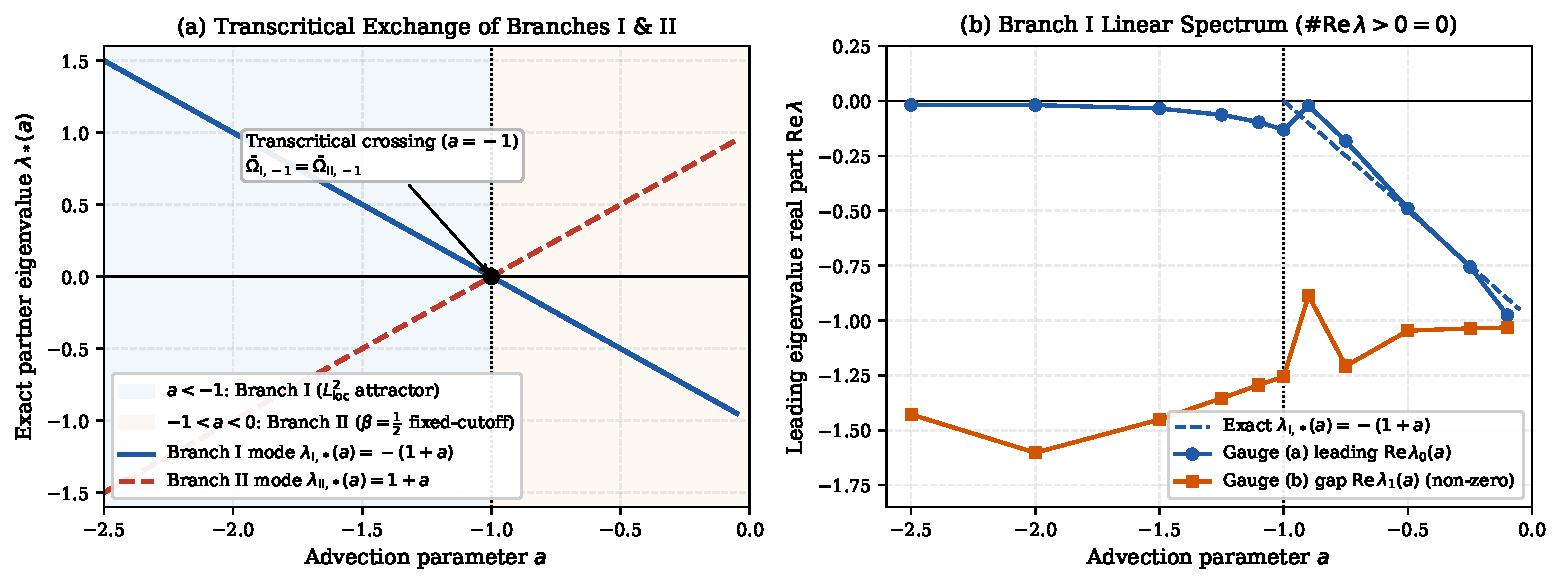
\includegraphics[width=\textwidth]{figures_gclm/fig1_gclm_branches_and_spectra.pdf}
\caption{(a) Transcritical exchange between Branch~I ($\gamma_{\mathrm{I}} = 1-a$, $\lambda_{\mathrm{I},*} = -(1+a)$) and Branch~II ($\gamma_{\mathrm{II}} = 2$, $\lambda_{\mathrm{II},*} = 1+a$) at $a = -1$. (b) Computed linear stability spectrum of Branch~I across $a \in [-2.5, -0.1]$ in Gauges~(a) and~(b) (\texttt{upwind2}, Gate~2), confirming $\#\{\operatorname{Re}\lambda > 0\} = 0$ and matching exact $\lambda_{\mathrm{I},*}(a) = -(1+a)$ on $-1 \le a < 0$.}
\label{fig:branches_spectra}
\end{figure}

\begin{numthm}[Certified Linear Stability Spectra $\lambda(a)$ Across $a < 0$; Gates~1--2 \& Gate~4 {[5]}]\label{numthm:spectra}
Discretizing the linearized Branch~I operator on edge-resolved $z = \ln(X-1)$ grids ($a \le -1$) and exact characteristic $\zeta = \ln(1 + v^\mu/|\cos\pi\mu|)$ grids ($-1 < a < 0$) with panel-exact Hilbert quadrature and second-order upwind advection (\texttt{upwind2}):
\begin{enumerate}
  \item \emph{Exact steady-state and nonlinear-FD agreement:} Branch~I and Branch~II steady residuals satisfy $\max|R_{\mathrm{ss}}| \le 6.5\times 10^{-16}$ (Gate~1) and $\le 2.0\times 10^{-16}$ ($1.91\times 10^{-16}$, Gate~3). Linearized operators match raw nonlinear dynamic-rescaling finite differences to $\le 9.2\times 10^{-12}$ (Gauge~a) and $\le 4.3\times 10^{-11}$ (Gauge~b) across $a \in [-2.0,-0.2]$ (Gate~2).
  \item \emph{Nyquist artifact diagnostic:} Central differencing introduces spurious unstable eigenvalues ($\lambda_0 = +0.991$ at $a=-1$ with Nyquist ratio $1.83$; $O(N)$-divergent edge mode $+4.78 \to +8.59$ at $a=-0.75$) because order-zero $H_+[g]$ destabilizes zero-group-velocity grid oscillations; \texttt{upwind2} eliminates these artifacts cleanly.
  \item \emph{Full stability across $a \in [-2.5, -0.1]$:} $\#\{\operatorname{Re}\lambda > 10^{-4}\} = 0$ across all tested $a$ in both Gauges~(a) and~(b) and across refinement/domain-depth sweeps (Figure~\ref{fig:branches_spectra}b). On $-1 < a < 0$, Gauge~(a) recovers $\lambda_{\mathrm{I},*}(a) = -(1+a)$ (e.g. $-0.50004$ vs $-0.50000$ at $a=-0.5$), while Gauge~(b) opens a uniform spectral gap $\operatorname{Re}\lambda_1 \approx -1.02$ to $-1.09$.
  \item \emph{Weighted semigroup contraction:} In Gauge~(b) on $\ker L_0$, the full $(N-1)$-dimensional restricted operator norm in $L^2_{1/2}(d\zeta)$ satisfies $\|e^{\tau M_a}|_{\ker L_0}\|_{L^2_{1/2}} e^{\tau/2} \le 0.99985 < 1$ for $a \in \{-0.25, -0.50, -0.75\}$ and $\tau = 1,\dots,4$ (Gate~4 {[5]}).
\end{enumerate}
\end{numthm}

%% ============================================================================
\section{Theorem~\ref{thm:conjugation}: Exact Two-Gamma Conjugation for \texorpdfstring{$M_c$}{Mc}}\label{sec:thm1}
%% ============================================================================

\begin{thm}[Exact 2-Gamma Conjugation and Slit-Plane Hardy Semigroup for $M_c$]\label{thm:conjugation}
For every $a < 0$, let
\[
\tilde c_{\mathrm{II},a}(r) := \left(\frac{1}{|a|} - \frac{1}{2r+1}\right)\tan(\pi r) = -\frac{2r + 1 + a}{a(2r+1)}\tan(\pi r),
\]
which is the exact Mellin symbol of $e^{+z/2}(\frac{1}{a}\widetilde{H}_0 + \frac{1}{2}\widetilde{Q}_0)$ throughout $\frac{1}{2} < \operatorname{Re} r < \frac{3}{2}$ (Lemma~\ref{lem:mellin}). Define the explicit 2-Gamma multiplier
\begin{equation}\label{eq:NL_II}
N_{L,\mathrm{II}}(s; a) := \sin(\pi s)\,|a|^{-2s}\,\frac{\Gamma(2s + 2 + a)}{\Gamma(2s + 2)},
\end{equation}
which reduces at $a = -1$ to the elementary function $N_{L,\mathrm{II}}(s;-1) = \frac{\sin(\pi s)}{2s+1}$. Fix $(a, \sigma)$ in the shift-strip pole-free regime:
\[
\text{either } a \in (-2, 0) \text{ and } \sigma \in \big(0, \tfrac{1}{2}\big), \qquad \text{or } a \in (-3, -2] \text{ and } \sigma \in \big(-1 - \tfrac{a}{2},\, \tfrac{1}{2}\big).
\]
Then:
\begin{enumerate}
  \item \textbf{Exact shift identity:} $N_{L,\mathrm{II}}(s;a)\,\tilde c_{\mathrm{II},a}(s+\frac{1}{2}) = -N_{L,\mathrm{II}}(s+\frac{1}{2};a)$ meromorphically on $\mathbb{C}$.
  \item \textbf{Stirling asymptotics and pole-free shift strip:} $N_{L,\mathrm{II}}(s;a)$ is analytic and zero-free on the closed shift strip $\sigma \le \operatorname{Re} s \le \sigma + \frac{1}{2}$, with two-sided Stirling bounds on $\operatorname{Re} s = \sigma$:
  \[
  c(\sigma,a)(1+|\xi|)^a e^{\pi|\xi|} \le |N_{L,\mathrm{II}}(\sigma+i\xi;a)| \le C(\sigma,a)(1+|\xi|)^a e^{\pi|\xi|}.
  \]
  \item \textbf{Explicit slit-plane Hardy contraction semigroup and exact spectrum:} Let $\mathcal{H}_{\sigma,a} := \mathcal{N}_{L,\mathrm{II}}^{-1}(L^2_\sigma(\mathbb{R}))$ with norm $\|G\|_{\mathcal{H}_{\sigma,a}} := \|\mathcal{N}_{L,\mathrm{II}} G\|_{L^2_\sigma(\mathbb{R})}$ (by Paley--Wiener, elements of $\mathcal{H}_{\sigma,a}$ extend analytically to $|\operatorname{Im} z| < \pi$, i.e.\ the slit plane $X \in \mathbb{C}\setminus(-\infty,1]$). On the dense domain $D(M_c) := \mathcal{N}_{L,\mathrm{II}}^{-1}(H^1_\sigma(\mathbb{R}) \cap L^2_{\sigma+1/2}(\mathbb{R}))$, the Gauge-(c) operator $M_c$ satisfies
  \[
  \mathcal{N}_{L,\mathrm{II}}\,M_c\,\mathcal{N}_{L,\mathrm{II}}^{-1} = A_\sigma := -2\partial_z - e^{-z/2} \quad \text{on } D(A_\sigma) := H^1_\sigma(\mathbb{R}) \cap L^2_{\sigma+1/2}(\mathbb{R}),
  \]
  and generates the explicit $C_0$-contraction semigroup
  \[
  e^{\tau M_c} = \mathcal{N}_{L,\mathrm{II}}^{-1}\,S(\tau)\,\mathcal{N}_{L,\mathrm{II}}, \qquad (S(\tau)F)(z) := \exp\!\Big(-e^{-z/2}(e^\tau - 1)\Big)\,F(z - 2\tau),
  \]
  with $\|e^{\tau M_c}\|_{\mathcal{H}_{\sigma,a}\to\mathcal{H}_{\sigma,a}} \le e^{-2\sigma\tau}$ ($\tau \ge 0$), exact spectrum $\sigma(M_c|_{\mathcal{H}_{\sigma,a}}) = \{\operatorname{Re}\lambda \le -2\sigma\}$ (empty point spectrum in $\operatorname{Re}\lambda > -2\sigma$), and resolvent bound $\|(\lambda - M_c)^{-1}\|_{\mathcal{H}_{\sigma,a}} \le (\operatorname{Re}\lambda + 2\sigma)^{-1}$.
\end{enumerate}
\end{thm}

\begin{remark}[Gauge~(c) vs.\ Gauge~(a) and the $a = -3$ Pole Threshold]\label{rem:thm1_gauge}
On $\operatorname{Re} s = \sigma \in (0,\frac{1}{2})$, the shifted line $\operatorname{Re} r = \sigma + \frac{1}{2} \in (\frac{1}{2}, 1)$ lies across the simple pole $r = \frac{1}{2}$ of $\tan(\pi r)$ inside the Gauge-(c) strip $(\frac{1}{2}, \frac{3}{2})$. Consequently $\mathcal{N}_{L,\mathrm{II}}$ conjugates $M_c$ --- not Gauge~(a) $M_{\mathrm{II},a}^{\mathrm{bulk}}$ --- except at $a = -2$ where $M_c \equiv M_{\mathrm{II},-2}^{\mathrm{bulk}}$. For $a \ne -2$, $M_{\mathrm{II},a}^{\mathrm{bulk}} G - M_c G = (\frac{1}{a}+\frac{1}{2})\widetilde{H}_{\mathrm{edge}}[G] \notin L^2_\sigma(\mathbb{R})$ whenever $\widehat{G}(\frac{1}{2}) \ne 0$ (verified numerically in Gate~4 {[1]}). Moreover, for $a \le -3$, every shift strip $[\sigma, \sigma+\frac{1}{2}]$ with $\sigma \in (0,\frac{1}{2})$ contains a pole $s_n = -1 - \frac{a+n}{2}$ of $\Gamma(2s+2+a)$, blocking full-domain conjugation.
\end{remark}

\begin{proof}[Proof of Theorem~\ref{thm:conjugation}]
(1) Using $\tan(\pi(s+\frac{1}{2})) = -\cot(\pi s)$ and $a = -|a| < 0$,
\begin{align*}
\frac{N_{L,\mathrm{II}}(s+\frac{1}{2}; a)}{N_{L,\mathrm{II}}(s; a)}
&= \frac{\sin(\pi s + \frac{\pi}{2})}{\sin(\pi s)}\cdot |a|^{-1}\cdot \frac{\Gamma(2s + 3 + a)}{\Gamma(2s + 2 + a)}\cdot \frac{\Gamma(2s + 2)}{\Gamma(2s + 3)} \\
&= \cot(\pi s)\,\frac{2s + 2 + a}{|a|(2s + 2)} = -\tilde c_{\mathrm{II},a}\!\left(s + \tfrac{1}{2}\right).
\end{align*}
(2) Zeros of $\sin(\pi s)$ lie at $\mathbb{Z}$, outside $[\sigma,\sigma+\frac{1}{2}] \subset (0,1)$; $\Gamma(2s+2)$ is zero- and pole-free on $\operatorname{Re} s > -1$; poles of $\Gamma(2s+2+a)$ lie at $s_n = -1 - \frac{a+n}{2}$ ($n \in \mathbb{N}_0$), with rightmost pole $s_0 = -1 - \frac{a}{2} < \sigma$ in both specified regimes. Stirling's formula gives $|\Gamma(2\sigma+2+a+2i\xi)/\Gamma(2\sigma+2+2i\xi)| = (2|\xi|)^a(1 + O(|\xi|^{-1}))$, while $|\sin(\pi(\sigma+i\xi))| \asymp e^{\pi|\xi|}$ on $\sigma \in (0,\frac{1}{2})$.

(3) Conjugating $S(\tau)$ by the unitary map $(U_\sigma F)(z) = e^{-\sigma z}F(z)$ from $L^2_\sigma(\mathbb{R})$ to $L^2(\mathbb{R})$ gives $(S_\sigma(\tau)u)(z) = e^{-2\sigma\tau}\exp(-e^{-z/2}(e^\tau - 1))u(z-2\tau)$, a strongly continuous semigroup on $L^2(\mathbb{R})$ with $\|S_\sigma(\tau)\|_{L^2\to L^2} \le e^{-2\sigma\tau}$ and closed generator $B_\sigma = -2\partial_z - 2\sigma - e^{-z/2}$ on $D(B_\sigma) = \{u \in H^1(\mathbb{R}) : e^{-z/2}u \in L^2(\mathbb{R})\}$. Pulling back via $U_\sigma^{-1}$ gives $D(A_\sigma) = H^1_\sigma(\mathbb{R}) \cap L^2_{\sigma+1/2}(\mathbb{R})$. For $F \in D(A_\sigma)$, $\widehat{F}(s)$ is analytic on $\sigma < \operatorname{Re} s < \sigma + \frac{1}{2}$ with $L^2$ boundary traces on both edges, and $\widehat{A_\sigma F}(s) = -2s\widehat{F}(s) - \widehat{F}(s+\frac{1}{2})$ on $\operatorname{Re} s = \sigma$. Setting $G := \mathcal{N}_{L,\mathrm{II}}^{-1} F$, analyticity and non-vanishing of $N_{L,\mathrm{II}}$ on $[\sigma,\sigma+\frac{1}{2}]$ imply $\widehat{G} = \widehat{F}/N_{L,\mathrm{II}}$ has $L^2$ traces on $\operatorname{Re} s = \sigma$ and $\operatorname{Re} r = \sigma + \frac{1}{2} \in (\frac{1}{2}, 1)$. Applying~(1) yields
\[
\frac{\widehat{A_\sigma F}(s)}{N_{L,\mathrm{II}}(s;a)} = -2s\,\widehat{G}(s) + \tilde c_{\mathrm{II},a}\!\left(s + \tfrac{1}{2}\right)\widehat{G}\!\left(s + \tfrac{1}{2}\right) = \widehat{M_c G}(s) \qquad (\operatorname{Re} s = \sigma),
\]
proving $\mathcal{N}_{L,\mathrm{II}} M_c \mathcal{N}_{L,\mathrm{II}}^{-1} = A_\sigma$ on $D(A_\sigma)$. Hille--Yosida gives the resolvent bound and $\sigma(M_c) \subset \{\operatorname{Re}\lambda \le -2\sigma\}$. For the reverse inclusion, the $L^2(\mathbb{R})$-adjoint $B_\sigma^* = 2\partial_z - 2\sigma - e^{-z/2}$ admits the explicit eigenfunctions
\[
\psi_\lambda(z) := \exp\!\left(\frac{2\sigma + \bar\lambda}{2}z - e^{-z/2}\right) \in D(B_\sigma^*)\setminus\{0\} \qquad (\forall \operatorname{Re}\lambda < -2\sigma),
\]
which decay exponentially as $z \to +\infty$ and super-exponentially as $z \to -\infty$. Hence every $\lambda$ with $\operatorname{Re}\lambda < -2\sigma$ belongs to $\sigma(B_\sigma)$ (in fact the residual spectrum, since $B_\sigma u = \lambda u$ has only super-exponentially growing solutions $C e^{-\frac{2\sigma+\lambda}{2}z + e^{-z/2}} \notin L^2(\mathbb{R})$). Closedness of $\sigma(B_\sigma)$ completes $\sigma(M_c|_{\mathcal{H}_{\sigma,a}}) = \{\operatorname{Re}\lambda \le -2\sigma\}$.
\end{proof}

%% ============================================================================
\section{Theorem~\ref{thm:sobolev_coerc}: Unconditional Finite-Sobolev Coercivity for Branch~II}\label{sec:coercivity}
%% ============================================================================

\begin{lem}[Mellin Representations of $\widetilde{H}_0$ and $\widetilde{Q}_0$]\label{lem:mellin}
For $G \in L^2_\sigma(\mathbb{R})$ with $\sigma \in (\frac{1}{2}, \frac{3}{2})$:
\begin{enumerate}
  \item $T_{H_0} G := e^{+z/2}\widetilde{H}_0[G]$ is a bounded Fourier--Mellin multiplier on $L^2_\sigma(\mathbb{R})$ with symbol $-\tan(\pi r)$ on $\operatorname{Re} r = \sigma$ and exact norm
  \[
  \|T_{H_0}\|_{L^2_\sigma \to L^2_\sigma} = \max\!\big(|\tan(\pi\sigma)|,\, 1\big) =
  \begin{cases}
  |\tan(\pi\sigma)|, & \sigma \in (\frac{1}{2}, \frac{3}{4}) \cup (\frac{5}{4}, \frac{3}{2}), \\
  1, & \sigma \in [\frac{3}{4}, \frac{5}{4}].
  \end{cases}
  \]
  In particular, $\|T_{H_0}\|_{L^2_{5/8}\to L^2_{5/8}} = \cot(\frac{\pi}{8}) = \sqrt{2} + 1$.
  \item $T_{Q_0} G := e^{+z/2}\widetilde{Q}_0[G]$ has Mellin symbol $-\frac{2\tan(\pi r)}{2r+1}$ on $\operatorname{Re} r = \sigma \in (\frac{1}{2}, \frac{3}{2})$, obeys $\partial_z\widetilde{Q}_0[G] = \widetilde{H}_0[G] - \widetilde{Q}_0[G]$, and satisfies $\|T_{Q_0}\|_{L^2_{5/8}\to L^2_{5/8}} \le \frac{8}{9}(\sqrt{2}+1)$.
  \item For every $k \ge 0$, $\partial_z^k\widetilde{H}_0[G] = e^{-z/2}T_{H_0}((\partial_z - \frac{1}{2})^k G)$ and $\partial_z^k\widetilde{Q}_0[G] = e^{-z/2}T_{Q_0}((\partial_z - \frac{1}{2})^k G)$.
\end{enumerate}
\end{lem}
\begin{proof}
Since $(T_{H_0}G)(\ln v) = v^{3/2}H_+[v^{-3/2}G](1+v)$ is a multiplicative convolution on $(0,\infty)$, its Mellin symbol on $\operatorname{Re} r = \sigma$ is $\frac{1}{\pi}\mathrm{P.V.}\int_0^\infty \frac{u^{3/2-r-1}}{u-1}\,du = -\cot(\pi(\frac{3}{2}-r)) = -\tan(\pi r)$ throughout the Muckenhoupt $A_2$ strip $0 < \frac{3}{2} - \sigma < 1 \iff \sigma \in (\frac{1}{2}, \frac{3}{2})$. Monotonicity of $|\tan(\pi(\sigma+i\xi))|^2 = \frac{\cosh(2\pi\xi)-\cos(2\pi\sigma)}{\cosh(2\pi\xi)+\cos(2\pi\sigma)}$ in $\cosh(2\pi\xi) \ge 1$ yields the exact norm. Part~(3) follows from exact dilation commutation $\partial_z H_+ = H_+ \partial_z$ on $(0,\infty)$.
\end{proof}

\begin{thm}[Unconditional Finite-Sobolev $H^k_\sigma$ Coercivity of $M_c$ for All $a \in [-2,0)$]\label{thm:sobolev_coerc}
Let $a \in [-2, 0)$ and $M_c = -2\partial_z + \frac{1}{a}\widetilde{H}_0 + \frac{1}{2}\widetilde{Q}_0$.
\begin{enumerate}
  \item \textbf{Exact $L^2_{1/4}$ energy identity} (for $G \in H^1_{1/4}(\mathbb{R}) \cap L^2_{5/8}(\mathbb{R})$):
  \begin{equation}\label{eq:L2_quarter_id}
  \begin{aligned}
  \langle M_c G,\, G\rangle_{L^2_{1/4}}
  &= -\frac{1}{2}\|G\|_{L^2_{1/4}}^2 - \frac{2-|a|}{4\pi|a|}\,\widehat{G}\!\left(\tfrac{1}{2}\right)^2
     - \frac{1}{4\pi}\int_{-\infty}^\infty \frac{\xi\coth(\pi\xi)}{1+\xi^2}\,\big|\widehat{G}(\tfrac{1}{2}+i\xi)\big|^2\,d\xi \\
  &\le -\frac{1}{2}\|G\|_{L^2_{1/4}}^2.
  \end{aligned}
  \end{equation}
  \item \textbf{Higher-order Plancherel coercivity:} For every $\sigma \in (\frac{1}{4}, \frac{3}{4})$ ($\sigma_1 := \sigma + \frac{1}{4} \in (\frac{1}{2}, 1)$), $k \in \mathbb{N}_0$, and $G \in H^{k+1}_\sigma(\mathbb{R}) \cap H^{k+1}_{\sigma_1}(\mathbb{R})$,
  \[
  \langle \partial_z^k M_c G,\, \partial_z^k G\rangle_{L^2_\sigma} = -2\sigma\|\partial_z^k G\|_{L^2_\sigma}^2 + \frac{1}{2\pi}\int_{-\infty}^\infty \operatorname{Re}\!\Big[(r-\tfrac{1}{2})^k\bar r^k\,\tilde c_{\mathrm{II},a}(r)\Big]|\widehat{G}(r)|^2\,d\xi,
  \]
  where $r = \sigma_1 + i\xi$. For \textbf{every $a \in [-2,0)$} and \textbf{every $\xi \in \mathbb{R}$}, $\operatorname{Re}[(r-\frac{1}{2})^k\bar r^k\tilde c_{\mathrm{II},a}(r)] < 0$ for $(\sigma = \frac{3}{8}, k \in \{0,1,2\})$ and $(\sigma = \frac{5}{8}, k \in \{0,1,2,3\})$, giving
  \begin{align*}
  \langle \partial_z^k M_c G,\, \partial_z^k G\rangle_{L^2_{3/8}} &\le -\frac{3}{4}\|\partial_z^k G\|_{L^2_{3/8}}^2 \quad (k\le 2), \\
  \langle \partial_z^k M_c G,\, \partial_z^k G\rangle_{L^2_{5/8}} &\le -\frac{5}{4}\|\partial_z^k G\|_{L^2_{5/8}}^2 \quad (k\le 3).
  \end{align*}
  At $\sigma = \frac{1}{4}$ ($\sigma_1 = \frac{1}{2}$), $\langle \partial_z^k M_c G, \partial_z^k G\rangle_{L^2_{1/4}} \le -\frac{1}{2}\|\partial_z^k G\|_{L^2_{1/4}}^2$ for $k = 0,1,2$ and all $a \in [-\frac{8}{5}, 0)$ (including $a = -1$).
\end{enumerate}
\end{thm}

\begin{proof}
(1) Symmetrizing $\langle \widetilde{H}[G], G\rangle_{L^2_{1/4}} = \frac{1}{\pi}\iint \frac{f(v)f(v')}{v(v-v')}\,dv\,dv'$ ($f = v^{-1/2}G$) via $\frac{1}{v(v-v')} + \frac{1}{v'(v'-v)} = -\frac{1}{vv'}$ gives $-\frac{1}{2\pi}\widehat{G}(\frac{1}{2})^2$. Subtracting $\widetilde{H}_{\mathrm{edge}}[G] = -\frac{1}{\pi}\widehat{G}(\frac{1}{2})$ adds $+\frac{1}{\pi}\widehat{G}(\frac{1}{2})^2$, so $\frac{1}{a}\langle \widetilde{H}_0[G], G\rangle_{L^2_{1/4}} = -\frac{1}{2\pi|a|}\widehat{G}(\frac{1}{2})^2$. For $\frac{1}{2}\widetilde{Q}_0$, shifting $\operatorname{Re} r = \frac{1}{2}+\epsilon \to \frac{1}{2}^+$ picks up the Sokhotski--Plemelj residue $+\frac{1}{4\pi}\widehat{G}(\frac{1}{2})^2$ from $-\frac{\tan(\pi r)}{2r+1}$ plus $-\frac{1}{4\pi}\int \frac{\xi\coth(\pi\xi)}{1+\xi^2}|\widehat{G}(\frac{1}{2}+i\xi)|^2\,d\xi$. Summing yields $\frac{1}{4\pi} - \frac{1}{2\pi|a|} = -\frac{2-|a|}{4\pi|a|} \le 0$ for $|a| \le 2$.

(2) Integration by parts gives $\langle -2\partial_z(\partial_z^k G), \partial_z^k G\rangle_{L^2_\sigma} = -2\sigma\|\partial_z^k G\|_{L^2_\sigma}^2$, while Lemma~\ref{lem:mellin}(3) gives the Plancherel formula on $\operatorname{Re} r = \sigma_1 = \sigma + \frac{1}{4}$. Set $P_k(\xi) := (r-\frac{1}{2})^k\bar r^k = ((\xi^2 + c) + \frac{i}{2}\xi)^k = R_k(x) + i\xi I_k(x)$ with $x := \xi^2 \ge 0$, $c := \sigma_1(\sigma_1-\frac{1}{2})$. (As $|\xi|\to\infty$, $\operatorname{Re}[P_k\tilde c_{\mathrm{II},a}] = -\frac{k+|a|}{2|a|}|\xi|^{2k-1} + O(|\xi|^{2k-3})$.)

\emph{Case $\sigma_1 = \frac{1}{2}$ ($k=1,2$):} The factor $(r-\frac{1}{2})^k = (i\xi)^k$ cancels the pole of $\tan(\pi r)$ at $r=\frac{1}{2}$ (no delta residue). Direct multiplication yields $\xi\coth(\pi\xi)(-\frac{1}{2|a|} + \frac{\frac{1}{2}-\xi^2}{2(1+\xi^2)}) \le 0$ for $k=1, |a|\le 2$, and $\xi^3\coth(\pi\xi)(-\frac{1}{|a|} + \frac{\frac{5}{4}-\xi^2}{2(1+\xi^2)}) \le 0$ for $k=2, |a|\le \frac{8}{5}$.

\emph{Case $\sigma_1 \in \{\frac{5}{8}, \frac{7}{8}\}$ (pure algebraic certificate for all $a \in [-2,0)$ and all $\xi \in \mathbb{R}$):} Decompose affinely in $\frac{1}{|a|} - \frac{1}{2} \ge 0$:
\[
\operatorname{Re}[P_k(\xi)\tilde c_{\mathrm{II},a}(r)] = \left(\frac{1}{|a|} - \frac{1}{2}\right)A_k(\xi) + \Big(\tfrac{1}{2}A_k(\xi) + B_k(\xi)\Big),
\]
where $\sin(2\pi\sigma_1) = -\frac{\sqrt{2}}{2}$, $D(\xi) := \cos(2\pi\sigma_1) + \cosh(2\pi\xi) > 0$, $d := 2\sigma_1 + 1 \in \{\frac{9}{4}, \frac{11}{4}\}$, and $\frac{1}{2} - \frac{1}{2r+1} = \frac{d(d-2)+4x+4i\xi}{2(d^2+4x)}$. Writing $U_k(x) + i\xi V_k(x) := (R_k(x) + i\xi I_k(x))(d(d-2) + 4x + 4i\xi)$ yields
\[
A_k(\xi) = -\frac{\frac{\sqrt{2}}{2}R_k(x) + \xi\sinh(2\pi\xi)I_k(x)}{D(\xi)}, \qquad
\frac{1}{2}A_k(\xi) + B_k(\xi) = -\frac{\frac{\sqrt{2}}{2}U_k(x) + \xi\sinh(2\pi\xi)V_k(x)}{2 D(\xi)(d^2 + 4x)}.
\]
In all seven cases ($\sigma_1 = \frac{5}{8}, k\le 2$; $\sigma_1 = \frac{7}{8}, k\le 3$), $R_k(x) > 0$ (at $\sigma_1 = \frac{5}{8}, k=2$, $R_2(x) = (x-\frac{3}{64})^2 + \frac{1}{256} > 0$; all other $R_k$ have strictly positive coefficients), $I_k(x) \ge 0$, and every coefficient of $V_k(x)$ is strictly positive, giving $A_k(\xi) < 0$ and $V_k(x) > 0$. Applying $\xi\sinh(2\pi\xi) \ge 2\pi x > 6x$ and $\frac{7}{10} < \frac{\sqrt{2}}{2} < \frac{3}{4}$ reduces positivity of the second numerator to the exact rational polynomial lower bound $W_{k,\mathrm{lb}}(x) := \sum_j (\alpha_j U_{k,j} + 6 V_{k,j-1})x^j$ ($\alpha_j = \frac{7}{10}$ if $U_{k,j} \ge 0$, $\frac{3}{4}$ if $U_{k,j} < 0$), every coefficient of which is strictly positive:
\begin{align*}
\sigma_1 = \tfrac{5}{8}:\quad & W_{0,\mathrm{lb}} = \tfrac{63}{160} + \tfrac{134}{5}x, \qquad W_{1,\mathrm{lb}} = \tfrac{63}{2048} + \tfrac{87}{32}x + \tfrac{194}{5}x^2, \\
& W_{2,\mathrm{lb}} = \tfrac{315}{131072} + \tfrac{633}{4096}x + \tfrac{9}{64}x^2 + \tfrac{254}{5}x^3; \\
\sigma_1 = \tfrac{7}{8}:\quad & W_{0,\mathrm{lb}} = \tfrac{231}{160} + \tfrac{134}{5}x, \qquad W_{1,\mathrm{lb}} = \tfrac{4851}{10240} + \tfrac{601}{40}x + \tfrac{194}{5}x^2, \\
& W_{2,\mathrm{lb}} = \tfrac{101871}{655360} + \tfrac{27081}{4096}x + \tfrac{1905}{64}x^2 + \tfrac{254}{5}x^3, \\
& W_{3,\mathrm{lb}} = \tfrac{2139291}{41943040} + \tfrac{169533}{65536}x + \tfrac{29433}{2048}x^2 + \tfrac{681}{16}x^3 + \tfrac{314}{5}x^4.
\end{align*}
Each of these seven inequalities (with $R_k, I_k, U_k, V_k$ derived recursively by \texttt{ring}) is also machine-checked over $\mathbb{R}$ in Lean~4 (\texttt{lem22\_cert\_58\_k0..2}, \texttt{lem22\_cert\_78\_k0..3}) and in exact Python \texttt{Fraction} arithmetic (Gate~4 {[2]}; see Figure~\ref{fig:coercivity_closure}a).
\end{proof}

\begin{figure}[t]
\centering
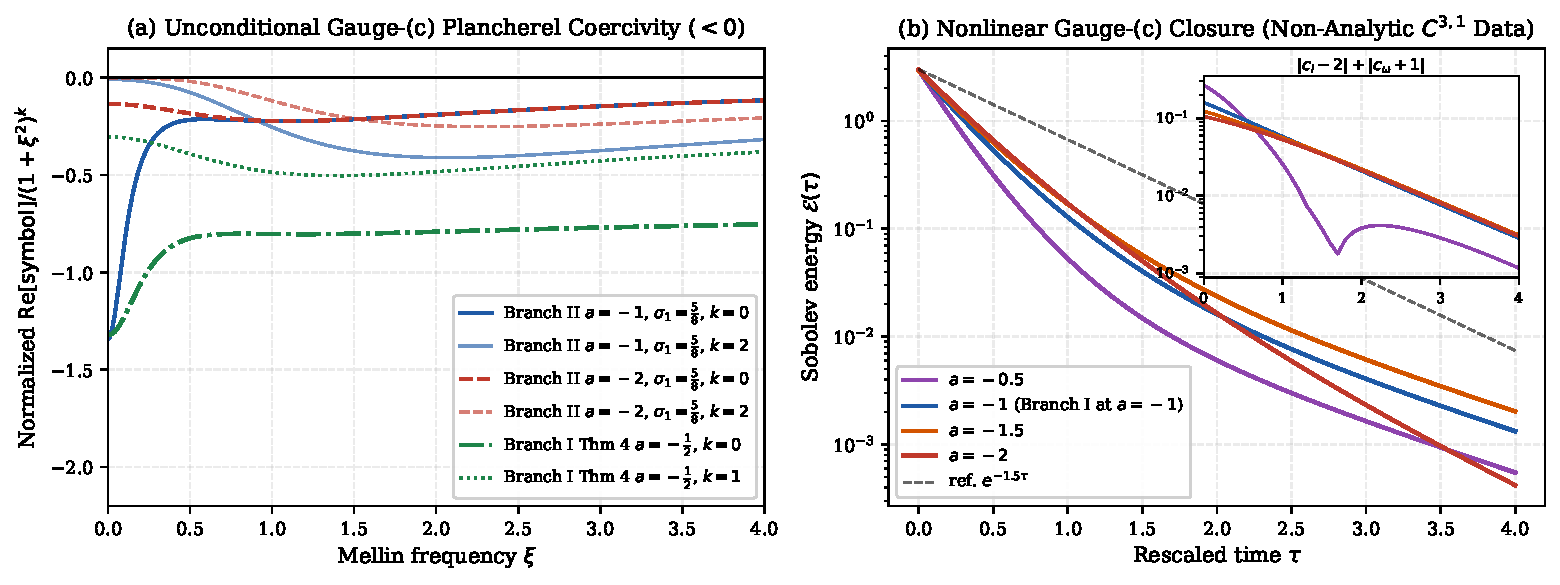
\includegraphics[width=\textwidth]{figures_gclm/fig2_gclm_coercivity_and_closure.pdf}
\caption{(a) Unconditional strict negativity of Gauge-(c) Plancherel symbols for Branch~II (Theorem~\ref{thm:sobolev_coerc}, $\sigma_1=\frac{5}{8}$) and Branch~I (Theorem~\ref{thm:branch1_h1}, $a = -\frac{1}{2}$). (b) Cancellation-free nonlinear Gauge-(c) evolution of the non-analytic $C^{3,1}$ compactly supported bump $G_0(z) = 0.2(1-(z/2)^2)_+^4$ ($\widehat{G}_0(\frac{1}{2}) \ne 0$) across $a \in \{-0.5, -1.0, -1.5, -2.0\}$ (Gate~4 {[4]}), showing strict monotonic exponential decay of $\mathcal{E}(\tau)$ and $(c_l, c_\omega) \to (2,-1)$ (inset).}
\label{fig:coercivity_closure}
\end{figure}

\begin{lem}[Far-Field $L^2([0,\infty))$, Scalar Functional, and Global $L^\infty$ Bounds]\label{lem:farfield}
For every $G \in H^2_{\sigma_-}(\mathbb{R}) \cap H^3_{5/8}(\mathbb{R})$ with $\sigma_- \in \{\frac{1}{4}, \frac{3}{8}\}$:
\begin{enumerate}
  \item With $C_{\sigma_-} := \cot(\pi(\frac{1}{2}-\sigma_-))$ ($C_{1/4} = 1$, $C_{3/8} = \sqrt{2}+1$),
  \[
  \|\partial_z^k\widetilde{H}[G]\|_{L^2([0,\infty),dz)} \le C_{\sigma_-}\|(\partial_z - \tfrac{1}{2})^k G\|_{L^2_{\sigma_-}(\mathbb{R})} \qquad (k = 0,1,2).
  \]
  Furthermore, the constant $\widetilde{H}_{\mathrm{edge}}[G]$ cancels identically in $\partial_z^m\widetilde{H}_0 = \partial_z^m\widetilde{H}$ ($m\ge 1$), $\partial_z\widetilde{Q}_0 = \widetilde{H} - \widetilde{Q}$, and $\partial_z^2\widetilde{Q}_0 = \partial_z\widetilde{H} - \widetilde{H} + \widetilde{Q}$, giving
  \[
  \|\widetilde{Q}[G]\|_{L^2([0,\infty))} + \sum_{m=1}^2\Big(\|\partial_z^m\widetilde{H}_0[G]\|_{L^2([0,\infty))} + \|\partial_z^m\widetilde{Q}_0[G]\|_{L^2([0,\infty))}\Big) \le C\big(\|G\|_{H^2_{\sigma_-}} + \|G\|_{H^2_{5/8}}\big).
  \]
  \item $|V_G| \le C_{V,\sigma_-}\|G\|_{L^2_{\sigma_-}}$ (with $C_{V,1/4} \approx 0.51036$, $C_{V,3/8} \approx 0.65136$) and $|\widetilde{H}_{\mathrm{edge}}[G]| \le \frac{1}{\pi}(2\|G\|_{L^2_{5/8}} + (1-2\sigma_-)^{-1/2}\|G\|_{L^2_{\sigma_-}})$.
  \item $\sum_{j=0}^1(\|\partial_z^j\widetilde{H}_0[G]\|_{L^\infty(\mathbb{R})} + \|\partial_z^j\widetilde{Q}_0[G]\|_{L^\infty(\mathbb{R})}) + \|\partial_z^2\widetilde{Q}_0[G]\|_{L^\infty(\mathbb{R})} \le C_*(\|G\|_{H^2_{\sigma_-}} + \|G\|_{H^3_{5/8}})$.
\end{enumerate}
\end{lem}
\begin{proof}
For~(1), on $v \ge 1$ we have $v^{-1} \le v^{-2\sigma_-}$. Since $v^{-2\sigma_-} \in A_2((0,\infty))$ with exact $H_+$-norm $\max(\cot(\pi(\frac{1}{2}-\sigma_-)), 1) = C_{\sigma_-}$ for $\sigma_- \in [\frac{1}{4},\frac{1}{2})$, setting $f_k(v) := v^{-1/2}(\partial_z-\frac{1}{2})^k G(\ln v)$ yields
\begin{align*}
\int_0^\infty |\partial_z^k\widetilde{H}[G]|^2\,dz
&= \int_1^\infty v^{-1}|H_+[f_k]|^2\,dv
\le C_{\sigma_-}^2\int_0^\infty v^{-2\sigma_--1}|(\partial_z-\tfrac{1}{2})^k G|^2\,dv \\
&= C_{\sigma_-}^2\|(\partial_z-\tfrac{1}{2})^k G\|_{L^2_{\sigma_-}}^2.
\end{align*}
Using $\widetilde{Q}[G](z) = e^{-z}\widetilde{Q}[G](0) + \int_0^z e^{z'-z}\widetilde{H}[G](z')\,dz'$ and Young's inequality gives $\|\widetilde{Q}[G]\|_{L^2([0,\infty))} \le \frac{1}{\sqrt{2}}|\widetilde{Q}[G](0)| + \|\widetilde{H}[G]\|_{L^2([0,\infty))}$, where $|\widetilde{Q}[G](0)| \le |(T_{Q_0}G)(0)| + |\widetilde{H}_{\mathrm{edge}}[G]| \le C(\|G\|_{L^2_{\sigma_-}} + \|G\|_{H^1_{5/8}})$ by Lemma~\ref{lem:mellin} and part~(2). Constant cancellation in $\partial_z^{1,2}\widetilde{Q}_0$ yields the remaining $L^2([0,\infty))$ bounds. Part~(2) is Cauchy--Schwarz, and part~(3) combines $e^{-z/2}|u(z)| \le \sqrt{2}\|u\|_{H^1_{5/8}}$ on $z \le 0$ with 1D Sobolev embedding on $[0,\infty)$ and parts~(1)--(2).
\end{proof}

%% ============================================================================
\section{Theorem~\ref{thm:nonlinear}: Zero-Analyticity Global Existence, Uniqueness, and Nonlinear Stability}\label{sec:nonlinear}
%% ============================================================================

\begin{thm}[Small-Data Finite-Sobolev Global Existence, Uniqueness, and Distributional Blowup]\label{thm:nonlinear}
Fix $a \in [-2, 0)$ (in particular $a = -1$, where $\bar\Omega_{\mathrm{I},-1} = \bar\Omega_{\mathrm{II},-1}$). Set $\sigma_- = \frac{3}{8}$ ($\lambda_0 = \frac{3}{4}$); if $a \in [-\frac{8}{5}, 0)$, all bounds below also hold with $\sigma_- = \frac{1}{4}$ ($\lambda_0 = \frac{1}{2}$) whenever $G_0 \in H^2_{1/4}(\mathbb{R})$. Define the finite-regularity Sobolev space
\[
\mathcal{X}_{\mathrm{gCLM}} := \Big\{G \in H^2_{\sigma_-}(\mathbb{R}) \cap H^3_{5/8}(\mathbb{R}) : G \in L^\infty([0,\infty)),\ \partial_z G \in H^1([0,\infty))\Big\},
\]
with weighted energy $\mathcal{E}(\tau) := \sum_{k=0}^2\|\partial_z^k G\|_{L^2_{\sigma_-}}^2 + \sum_{k=0}^3\|\partial_z^k G\|_{L^2_{5/8}}^2$ and far-field norm $\mathcal{B}(\tau) := \|G\|_{L^\infty([0,\infty))} + \|\partial_z G\|_{H^1([0,\infty))}$. There exist explicit $a$-dependent constants $\varepsilon_0 > 0$ and $M, C > 0$ such that for every initial datum $G_0 \in \mathcal{X}_{\mathrm{gCLM}}$ satisfying $\sqrt{\mathcal{E}(0)} + \mathcal{B}(0) \le \varepsilon_0$:
\begin{enumerate}
  \item \textbf{Unconditional global existence and uniqueness:} There exists a \textbf{unique} global solution
  \[
  \begin{aligned}
  G \in{} &C\big([0,\infty); H^1_{\sigma_-}(\mathbb{R}) \cap H^2_{5/8}(\mathbb{R})\big) \cap C_w\big([0,\infty); H^2_{\sigma_-}(\mathbb{R}) \cap H^3_{5/8}(\mathbb{R})\big) \\
          &\cap L^\infty\big([0,\infty); \mathcal{X}_{\mathrm{gCLM}}\big) \cap L^2\big([0,\infty); H^{5/2}_{7/8}(\mathbb{R})\big)
  \end{aligned}
  \]
  of~\eqref{eq:nonlin_gauge_c} with $G(\cdot,0) = G_0$ (constructed in Appendix~\ref{app:lwp} via Mellin-compatible weighted viscous regularization, Lions' parabolic theorem, and vanishing viscosity; uniqueness holds in the larger class $\cap\,L^2_{\mathrm{loc}}([0,\infty); L^2_{7/8}(\mathbb{R}))$).
  \item \textbf{Global exponential decay and parameter convergence:} For all $\tau \in [0,\infty)$,
  \[
  \mathcal{E}(\tau) \le \mathcal{E}(0)\,e^{-\lambda_0\tau}, \qquad \sqrt{\mathcal{E}(\tau)} + \mathcal{B}(\tau) \le \frac{M}{2}\varepsilon_0 < M\varepsilon_0, \qquad \lim_{z\to-\infty}G(z,\tau) = 0,
  \]
  and $|c_l(\tau) - 2| + |c_\omega(\tau) + 1| \le C\sqrt{\mathcal{E}(0)}\,e^{-\lambda_0\tau/2}$ (see Figure~\ref{fig:coercivity_closure}b).
  \item \textbf{Global conservative distributional blowup:} The reconstructed vorticity $\Omega(X,\tau) = \frac{1}{a}(X-1)^{-1/2}(1+G(\ln(X-1),\tau))\mathbf{1}_{\{X>1\}}$ solves~\eqref{eq:gclm_dyn} globally on $\mathbb{R}$ in conservative weak form with zero $\delta(X-1)$ defect (Proposition~\ref{prop:weak_form}) and converges uniformly on compact subsets of $(1,\infty)$ to $\bar\Omega_{\mathrm{II},a}$. In physical variables, at the finite time $T_* = \int_0^\infty C_\omega(\tau)\,d\tau < \infty$, the singular edge $x_{\mathrm{edge}}(t) = C_l(\tau(t))^{-1} \sim c_L(T_*-t)^2$ collapses to $x = 0$ with exact exponent $\gamma = 2$, while the self-similar amplitude blows up as $C_\omega(\tau(t))^{-1} \sim c_*(T_*-t)^{-1}$ (e.g.\ $u_x(0,t) \sim \frac{c_*}{|a|}(T_*-t)^{-1} \to +\infty$).
\end{enumerate}
\end{thm}

\begin{proof}[Proof of Theorem~\ref{thm:nonlinear} (Uniqueness and \emph{A Priori} Closure; Global Existence in Appendix~\ref{app:lwp})]
Set $F[G] := \frac{1}{a}\widetilde{H}_0[G] + \frac{1}{2}\widetilde{Q}_0[G]$ and $c(z,\tau) := 2 + \widetilde{Q}[G](z) - V_G$. By 1D Sobolev embedding on $(-\infty,0]$ and $[0,\infty)$, $\lim_{z\to-\infty}|G(z,\tau)| \le \lim_{z\to-\infty}\sqrt{2}e^{5z/8}\|G\|_{H^1_{5/8}} = 0$, and
\begin{equation}\label{eq:wlinf}
\|e^{-\alpha z}G\|_{L^\infty(\mathbb{R})} + \|e^{-\alpha z}\partial_z G\|_{L^\infty(\mathbb{R})} \le C(\sqrt{\mathcal{E}} + \mathcal{B}) \qquad \forall \alpha \in [0, \tfrac{5}{8}].
\end{equation}

\paragraph{Uniqueness in $L^\infty([0,T]; \mathcal{X}_{\mathrm{gCLM}}) \cap L^2_{\mathrm{loc}}([0,T]; L^2_{7/8}(\mathbb{R}))$.}
Let $W := G_1 - G_2$ for two solutions in $C([0,T]; H^1_{\sigma_-}\cap H^2_{5/8}) \cap L^\infty([0,T]; \mathcal{X}_{\mathrm{gCLM}}) \cap L^2([0,T]; L^2_{7/8}(\mathbb{R}))$ with equal data. Subtracting~\eqref{eq:nonlin_gauge_c} yields $\partial_\tau W = M_c W - (\widetilde{Q}[G_1] - V_{G_1})\partial_z W - (\widetilde{Q}_0[W] + \widetilde{H}_{\mathrm{edge}}[W] - V_W)\partial_z G_2 + F[G_1]W + F[W]G_2$. Testing against $W$ in $L^2_\sigma(\mathbb{R})$ for $\sigma \in \{\sigma_-, \frac{5}{8}\}$ (using the Gelfand triple $H^1_{5/8}\cap L^2_{7/8} \hookrightarrow L^2_{5/8} \hookrightarrow (H^1_{5/8}\cap L^2_{7/8})^*$ at $\sigma = \frac{5}{8}$, where $W \in L^2([0,T]; L^2_{7/8})$ guarantees absolute convergence of $\langle T_{\tilde c}W, W\rangle_{L^2_{7/8}}$): $\langle M_c W, W\rangle_{L^2_\sigma} \le 0$ (Theorem~\ref{thm:sobolev_coerc}); IBP and Lemma~\ref{lem:farfield} control the $G_1$ and scalar terms by $C(\sqrt{\mathcal{E}_1}+\sqrt{\mathcal{E}_2})(\|W\|_{L^2_{\sigma_-}}^2 + \|W\|_{L^2_{5/8}}^2)$; and writing $\widetilde{Q}_0[W] = e^{-z/2}T_{Q_0}W$, $F[W] = e^{-z/2}T_F W$ with the weight split $e^{-2\sigma z}e^{-z/2} = e^{-(\sigma-1/8)z}e^{-5z/8}e^{-\sigma z}$ ($\alpha = \sigma - \frac{1}{8} \in [\frac{1}{8},\frac{1}{2}] \subset [0,\frac{5}{8}]$) controls the remaining terms via~\eqref{eq:wlinf} by $C(\sqrt{\mathcal{E}_2}+\mathcal{B}_2)\|W\|_{L^2_{5/8}}\|W\|_{L^2_\sigma}$. Summing over $\sigma \in \{\sigma_-, \frac{5}{8}\}$ and applying Gronwall gives $W \equiv 0$.

\paragraph{Three-Block \emph{A Priori} Closure (Parts~(2)--(3)).}
Assume $\sqrt{\mathcal{E}(\tau)} + \mathcal{B}(\tau) \le M\varepsilon_0$, with $\varepsilon_0$ small enough that $C_* M\varepsilon_0 \le 1$ (hence $c(z,\tau) \ge 1$ on $\mathbb{R}$) and $M\varepsilon_0 \le \frac{1}{2}$.

\emph{Block 1 (Weighted energy $\mathcal{E}$):} Differentiating~\eqref{eq:nonlin_gauge_c} $k$ times ($k\le 2$ for $\sigma_-$, $k\le 3$ for $\sigma_+ = \frac{5}{8}$) and testing against $\partial_z^k G$ in $L^2_\sigma$:
(i) linear term $\langle \partial_z^k M_c G, \partial_z^k G\rangle_{L^2_\sigma} \le -2\sigma\|\partial_z^k G\|_{L^2_\sigma}^2 \le -\lambda_0\|\partial_z^k G\|_{L^2_\sigma}^2$ (Theorem~\ref{thm:sobolev_coerc}), plus the $\nu$-independent nonlocal $H^{5/2}_{7/8}$ dissipation $-c_0\|G\|_{H^{5/2}_{7/8}}^2$ from $k=3, \sigma=\frac{5}{8}$ (used in Appendix~\ref{app:lwp});
(ii) top-order advection $-\langle (\widetilde{Q}-V_G)\partial_z^{k+1}G, \partial_z^k G\rangle_{L^2_\sigma} \le C\sqrt{\mathcal{E}}\|\partial_z^k G\|_{L^2_\sigma}^2$ by IBP and Lemma~\ref{lem:farfield}(2)--(3) (zero derivative loss);
(iii) lower-order commutators ($1\le j\le k$) and stretching terms ($0\le j\le k$): for $j \le 1$ (and $j=2 < k$ for $\partial_z^2\widetilde{Q}_0[G]$), Lemma~\ref{lem:farfield}(3) gives $L^\infty$ bounds $\le C\sqrt{\mathcal{E}}$, yielding $\le C\mathcal{E}^{3/2}$; for top nonlocal derivatives $j \in \{2,3\}$ ($k-j \in \{0,1\}$, plus $j = k \in \{2,3\}$ for $\partial_z^j\widetilde{Q}_0[G]$), Lemma~\ref{lem:mellin}(3) gives $\partial_z^j\widetilde{Q}_0 = e^{-z/2}T_{Q_0}((\partial_z-\frac{1}{2})^j G)$ and $\partial_z^j F = e^{-z/2}T_F((\partial_z-\frac{1}{2})^j G)$ bounded in $L^2_{5/8}$ by $C\sqrt{\mathcal{E}}$, and splitting $e^{-2\sigma z}e^{-z/2} = e^{-(\sigma-1/8)z}e^{-5z/8}e^{-\sigma z}$ with~\eqref{eq:wlinf} yields $\le C(\sqrt{\mathcal{E}}+\mathcal{B})\mathcal{E}$. Summing over $k$ and multiplying by $2$ gives
\begin{equation}\label{eq:block1}
\frac{d}{d\tau}\mathcal{E} + 2 c_0\|G\|_{H^{5/2}_{7/8}}^2 \le -2\lambda_0\,\mathcal{E} + 2 C_{\mathrm{nl}}(\sqrt{\mathcal{E}} + \mathcal{B})\,\mathcal{E}.
\end{equation}

\emph{Block 2 (Far-field derivative energy $P := \|\partial_z G\|_{H^1([0,\infty))}^2$):} Testing $\partial_z^{m+1}$\eqref{eq:nonlin_gauge_c} against $\partial_z^{m+1}G$ on $[0,\infty)$ ($m \in \{0,1\}$): inflow IBP at $z=0$ contributes $\frac{1}{2}c(0,\tau)(\partial_z^{m+1}G(0,\tau))^2 \le C\mathcal{E}$ (since $H^3_{5/8} \hookrightarrow C^2$), while Lemma~\ref{lem:farfield}(1),(3) bounds $\|\partial_z^{m+1}F[G]\|_{L^2([0,\infty))} \le C\sqrt{\mathcal{E}}$ and all lower $L^\infty$ coefficients by $C\sqrt{\mathcal{E}}$. Summing $m=0,1$ yields $\frac{1}{2}\dot P \le C_1\mathcal{E} + C_2(1+\mathcal{B})\sqrt{\mathcal{E}}\sqrt{P} + C_3\sqrt{\mathcal{E}}P$. Whenever $\dot{\mathcal{E}} \le 0$, for any $\delta > 0$,
\[
\frac{d}{d\tau}\sqrt{P + \mathcal{E} + \delta^2} = \frac{\frac{1}{2}\dot P + \frac{1}{2}\dot{\mathcal{E}}}{\sqrt{P+\mathcal{E}+\delta^2}} \le C_4(1+\mathcal{B})\sqrt{\mathcal{E}}, \qquad C_4 := \max(C_1+C_2, C_2+C_3).
\]
Integrating and letting $\delta \to 0^+$ yields $\sqrt{P(\tau)} \le \sqrt{P(0)} + \sqrt{\mathcal{E}(0)} + C_4\int_0^\tau(1+\mathcal{B})\sqrt{\mathcal{E}}\,ds$.

\emph{Block 3 (Far-field amplitude $\|G\|_{L^\infty([0,\infty))}$):} Since $c \ge 1$ on $[0,\infty)$, every characteristic starts at $Z(0)\ge 0$ or enters at $Z(\tau_0) = 0$ with $|G(0,\tau_0)| \le C_0\sqrt{\mathcal{E}(\tau_0)}$, giving $\|G(\tau)\|_{L^\infty([0,\infty))} \le \|G_0\|_{L^\infty([0,\infty))} + C_0\sup_{s\le\tau}\sqrt{\mathcal{E}(s)} + C_5\int_0^\tau(1+\mathcal{B})\sqrt{\mathcal{E}}\,ds$.

\emph{Bootstrap closure and global existence:} Set $K := 1 + \sqrt{2} + C_0 + \frac{3(C_4'+C_5')}{\lambda_0}$ (using the viscous-compatible constants $C_4' \ge C_4$, $C_5' \ge C_5$ from Appendix~\ref{app:lwp}), $M := 2(1+K)$, and require $2 C_{\mathrm{nl}}M\varepsilon_0 \le \frac{\lambda_0}{2}$. Then~\eqref{eq:block1} gives $\mathcal{E}(\tau) \le \mathcal{E}(0)e^{-\lambda_0\tau}$ and $\int_0^\tau\sqrt{\mathcal{E}}\,ds \le \frac{2}{\lambda_0}\sqrt{\mathcal{E}(0)}$. Substituting into Blocks~2--3 (with $1+\mathcal{B}\le\frac{3}{2}$ and $2 < 1+\sqrt{2}$) gives $\sqrt{\mathcal{E}(\tau)} + \mathcal{B}(\tau) \le \mathcal{B}(0) + K\sqrt{\mathcal{E}(0)} \le (1+K)\varepsilon_0 = \frac{M}{2}\varepsilon_0 < M\varepsilon_0$, closing strictly. Appendix~\ref{app:lwp} constructs the global solution $G$ via the Mellin-compatible weighted viscous regularization $\mathcal{D}_\nu G = \nu(1+e^{-z/2})\partial_z^2 G - \nu e^{-z/2}G$, transferring all uniform bounds (including $G \in L^2([0,\infty); H^{5/2}_{7/8}(\mathbb{R}))$ and the $\sigma_- = \frac{1}{4}$ extension for $a \in [-\frac{8}{5}, 0)$ in Step~5) in the $\nu \to 0^+$ limit. Part~(3) follows from Proposition~\ref{prop:weak_form} and integrating $\frac{dt}{d\tau} = C_\omega(\tau) = \exp(-\tau + O(1))$, $C_l(\tau) = \exp(2\tau + O(1))$.
\end{proof}

%% ============================================================================
\section{Theorem~\ref{thm:branch1_h1}: Unconditional \texorpdfstring{$H^1_\sigma$}{H1\_sigma} Coercivity of Branch~I for All \texorpdfstring{$a \in [-1,0)$}{a in [-1,0)}}\label{sec:branch1_thm4}
%% ============================================================================

Although Branch~I admits no finite Gamma-product conjugator for $a \ne -1$, the same Gauge-(c) reduction yields an elementary coercivity proof for every $a \in [-1,0)$. Setting $\mu = (1-a)^{-1} \in [\frac{1}{2}, 1)$, $\kappa = -\cos(\pi\mu) \ge 0$,
\begin{align*}
\widetilde{H}_{\mathrm{I}}[G](z) &:= -\sin(\pi\mu)\,H_+[v^{-\mu}G](1+e^z), &
\widetilde{Q}_{\mathrm{I}}[G](z) &:= \int_{-\infty}^z e^{z'-z}\widetilde{H}_{\mathrm{I}}[G](z')\,dz', \\
\widetilde{H}_{\mathrm{I},\mathrm{edge}}[G] &:= \frac{\sin(\pi\mu)}{\pi}\widehat{G}(\mu), &
V_{\mathrm{I},G} &:= \frac{a\sin(\pi\mu)}{\pi}\int_{\mathbb{R}} e^{(1-\mu)z}\ln(1+e^{-z})G(z)\,dz,
\end{align*}
Branch~I Gauge~(c) imposes $c_l = (1-a) - V_{\mathrm{I},G}$ and $c_\omega = -\mu c_l - \mu\widetilde{H}_{\mathrm{I},\mathrm{edge}}[G]$, yielding the linearized operator
\begin{equation}\label{eq:M_Ic}
M_{\mathrm{I},c} G := -(1-a)(1 + \kappa e^{-\mu z})\partial_z G + \widetilde{H}_{\mathrm{I},0}[G] - (1-\mu)\widetilde{Q}_{\mathrm{I},0}[G],
\end{equation}
where $\widetilde{H}_{\mathrm{I},0}[G]$ and $\widetilde{Q}_{\mathrm{I},0}[G]$ are defined directly on the entire Muckenhoupt strip $\sigma_1 \in (\mu, 1+\mu)$ by the subtracted kernels
\begin{align*}
\widetilde{H}_{\mathrm{I},0}[G](z) &:= -\frac{\sin(\pi\mu)\,e^z}{\pi}\mathrm{P.V.}\int_0^\infty \frac{(v')^{-1-\mu}G(\ln v')}{e^z - v'}\,dv', \\
\widetilde{Q}_{\mathrm{I},0}[G](z) &:= \int_{-\infty}^z e^{z'-z}\widetilde{H}_{\mathrm{I},0}[G](z')\,dz'
\end{align*}
(which coincide with $\widetilde{H}_{\mathrm{I}} - \widetilde{H}_{\mathrm{I},\mathrm{edge}}$ and $\widetilde{Q}_{\mathrm{I}} - \widetilde{H}_{\mathrm{I},\mathrm{edge}}$ whenever $\widehat{G}(\mu)$ converges).

\begin{thm}[Unconditional $H^1_\sigma(\mathbb{R})$ Coercivity of Huang--Tong--Wang's Branch~I for All $a \in [-1,0)$]\label{thm:branch1_h1}
Fix any $a \in [-1, 0)$ ($\mu = (1-a)^{-1} \in [\frac{1}{2},1)$, $\kappa = -\cos(\pi\mu) \ge 0$) and any $\theta \in (0,\frac{1}{2})$. Set $\sigma_1 := \mu + \theta$ and $\sigma := \sigma_1 - \frac{\mu}{2} = \frac{\mu}{2} + \theta \in (\frac{\mu}{2}, \frac{1+\mu}{2})$. Then for $k \in \{0,1\}$ and every $G \in H^{k+1}_\sigma(\mathbb{R}) \cap H^{k+1}_{\sigma_1}(\mathbb{R})$, the weighted bilinear form $\langle \partial_z^k M_{\mathrm{I},c} G, \partial_z^k G\rangle_{L^2_\sigma} := \int_{\mathbb{R}} e^{-2\sigma z}(\partial_z^k M_{\mathrm{I},c} G)(\partial_z^k G)\,dz$ converges absolutely (via $2\sigma + \mu = 2\sigma_1$) and satisfies, with $r = \sigma_1 + i\xi$:
\begin{enumerate}
  \item $\langle \partial_z^k M_{\mathrm{I},c} G,\, \partial_z^k G\rangle_{L^2_\sigma} = -(1-a)\sigma\|\partial_z^k G\|_{L^2_\sigma}^2 + \frac{1}{2\pi}\int_{\mathbb{R}} \operatorname{Re}[(r-\mu)^k\bar r^k c_a(\mu-r)]|\widehat{G}(r)|^2\,d\xi$.
  \item For every $\xi \in \mathbb{R}$,
  \begin{align*}
  \operatorname{Re}[c_a(\mu-r)]
  &= -(1-a)\kappa\sigma_1 \\
  &\quad - \sin(\pi\mu)\frac{\sin(2\pi\theta)(\sigma_1(1+\theta)+\xi^2) + (1-\mu)\xi\sinh(2\pi\xi)}{(\cosh(2\pi\xi)-\cos(2\pi\theta))((1+\theta)^2+\xi^2)} < 0, \\
  \operatorname{Re}[(r-\mu)\bar r\,c_a(\mu-r)]
  &= -(1-a)\kappa\theta|r|^2 \\
  &\quad - \sin(\pi\mu)|r|^2\frac{\sin(2\pi\theta)(\theta(1+\theta)+\xi^2) + \xi\sinh(2\pi\xi)}{(\cosh(2\pi\xi)-\cos(2\pi\theta))((1+\theta)^2+\xi^2)} < 0.
  \end{align*}
  \item Consequently, $\langle \partial_z^k M_{\mathrm{I},c} G, \partial_z^k G\rangle_{L^2_\sigma} \le -(1-a)\sigma\|\partial_z^k G\|_{L^2_\sigma}^2 - (1-a)\kappa(\sigma_1 - k\mu)\|\partial_z^k G\|_{L^2_{\sigma_1}}^2 \le -(1-a)\sigma\|\partial_z^k G\|_{L^2_\sigma}^2$ ($k = 0,1$). Choosing $\sigma_- = \frac{3\mu}{4} \in (\frac{\mu}{2},\mu)$ and $\sigma_+ = \frac{1+3\mu}{4} \in (\mu,\frac{1+\mu}{2})$ yields simultaneous $H^1_{\sigma_-}\cap H^1_{\sigma_+}$ coercivity and Cauchy--Schwarz boundedness of $V_{\mathrm{I},G}$ and $\widetilde{H}_{\mathrm{I},\mathrm{edge}}[G]$.
\end{enumerate}
\end{thm}
\begin{proof}
On the Muckenhoupt $A_2$ strip $\sigma_1 \in (\mu, 1+\mu)$, $e^{\mu z}(\widetilde{H}_{\mathrm{I},0} - (1-\mu)\widetilde{Q}_{\mathrm{I},0})$ has Mellin symbol $\sin(\pi\mu)\cot(\pi(\mu-r))\frac{r}{r+1-\mu}$. Combining with $-(1-a)\kappa e^{-\mu z}\partial_z G$ gives total $e^{-\mu z}$-shifted symbol $-(1-a)\kappa r + \sin(\pi\mu)\cot(\pi(\mu-r))\frac{r}{r+1-\mu} = c_a(\mu-r)$, proving~(1) by dilation commutation and Plancherel. Writing $r = \mu + \theta + i\xi$ gives $\cot(\pi(\mu-r)) = \frac{-\sin(2\pi\theta) + i\sinh(2\pi\xi)}{\cosh(2\pi\xi) - \cos(2\pi\theta)}$ with $\sin(2\pi\theta) > 0$. Both $\frac{r}{r+1-\mu} = \frac{\sigma_1(1+\theta)+\xi^2 + i(1-\mu)\xi}{(1+\theta)^2+\xi^2}$ ($k=0$) and $(r-\mu)\bar r\frac{r}{r+1-\mu} = |r|^2\frac{\theta(1+\theta)+\xi^2 + i\xi}{(1+\theta)^2+\xi^2}$ ($k=1$) have strictly positive real and imaginary coefficients for all $\xi \in \mathbb{R}$, proving~(2) and~(3) immediately.
\end{proof}

%% ============================================================================
\section{Nonlinear DNS Selection for \texorpdfstring{$a < -1$}{a < -1} and \texorpdfstring{$L^2$}{L2}-Criticality}\label{sec:dns}
%% ============================================================================

For $a < -1$, Branch~I has an interior repelling stagnation point $X_* = 1 + (\cos\pi\mu)^{1/\mu} > 1$ and an unstable steeper $L^1_{\mathrm{loc}}\setminus L^2_{\mathrm{loc}}$ mode $\lambda_{\mathrm{I},*}(a) = |a|-1 > 0$, while Branch~II has strictly outgoing advection $\bar A_{\mathrm{II}} = 2v > 0$ and a stable partner mode $\lambda_{\mathrm{II},*}(a) = 1+a < 0$. Which branch actually attracts smooth degenerate half-line initial data under the full nonlinear gCLM flow?

To answer this without artificial edge bias, we evolve the Case~2.2 dynamic-rescaling gCLM PDE~\eqref{eq:gclm_dyn} ($H(\Omega)(0,\tau) \equiv 1$, edge pinned at $X = 1$) on a stretched coordinate $v(\rho) = 10^{-4}(e^\rho - 1)$ ($\rho \in [0, 29]$, $v_{\max} \approx 3.9\times 10^8$) using fifth-order upwind WENO5, third-order SSP-RK3, and an exact logarithmic-kernel Hilbert operator $J(v) = \frac{1}{\pi}\int_0^\infty \Omega(1+v')\ln\big|\frac{v-v'}{v'}\big|\,dv'$ (Gate~3, \texttt{src/gclm\_singular/dns.py}).

\begin{figure}[t]
\centering
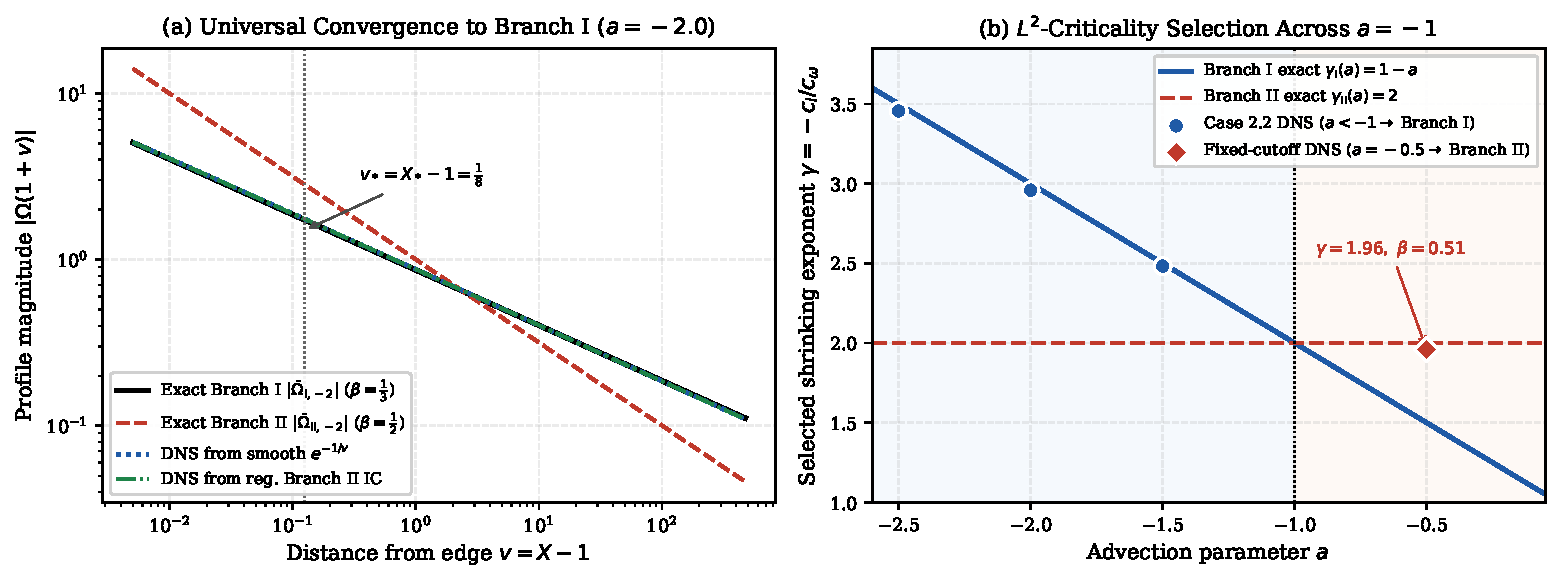
\includegraphics[width=\textwidth]{figures_gclm/fig3_gclm_dns_selection.pdf}
\caption{(a) Nonlinear Case~2.2 DNS at $a = -2.0$ from both smooth degenerate data ($\Omega_0 \propto -e^{-1/v}$) and regularized Branch~II data ($\Omega_0 \propto -(v+10^{-3})^{-1/2}$) collapsing identically onto Branch~I ($\beta = \frac{1}{3}$, $\gamma = 3.0$, $v_* = \frac{1}{8}$). (b) $L^2$-criticality selection across $a = -1$: Case~2.2 DNS selects Branch~I ($\gamma = 1-a$) for $a < -1$, whereas fixed-cutoff $X > 1$ DNS at $a = -0.5$ locks onto Branch~II ($\gamma = 2$, $\beta = \frac{1}{2}$).}
\label{fig:dns_selection}
\end{figure}

\begin{itemize}
  \item \textbf{Universal convergence to Branch~I for $a < -1$ (Figure~\ref{fig:dns_selection}a):} Across $a \in \{-1.5, -2.0, -2.5\}$, smooth degenerate initial data (\texttt{exp\_inv}, \texttt{poly\_exp}) \emph{and} regularized Branch~II initial data all converge universally to Branch~I with bulk residuals $\le 2.8\times 10^{-8}$ ($2.74\times 10^{-8}$ worst case), relative profile error $0.64\%$--$1.89\%$, exact interior stagnation point $X_*$, and universality spread $3.3\times 10^{-8}$ at $a = -2.0$.
  \item \textbf{The $L^2$-criticality selection mechanism (Figure~\ref{fig:dns_selection}b):} Integrating the Case~2.2 normalization condition $\frac{d}{d\tau}\int_1^\infty \frac{\Omega}{X}\,dX = 0$ by parts gives
  \[
  c_\omega = \frac{1+a}{\pi}\int_1^\infty \frac{U_X\Omega}{X}\,dX - \frac{a}{\pi}\int_1^\infty \frac{U\Omega}{X^2}\,dX + \text{(edge flux at } X = 1^+\text{)}.
  \]
  For Branch~I, $U_X\Omega \sim (X-1)^{-2\mu}$ is integrable at $X = 1^+$ \textbf{if and only if $2\mu < 1 \iff a < -1$} ($\bar\Omega_{\mathrm{I},a} \in L^2_{\mathrm{loc}}$). In this regime the edge flux vanishes identically and exact Beta integrals give $c_\omega = -1$ (verified to $5.55\times 10^{-16}$ in Gate~3 {[4]}), allowing smooth degenerate half-line data to form Branch~I smoothly. Conversely, for $-1 < a < 0$, $\bar\Omega_{\mathrm{I},a} \notin L^2_{\mathrm{loc}}$; enforcing a hard cutoff $\Omega \equiv 0$ on $X < 1$ without an inner traveling wave blocks Branch~I and forces the flow onto the $L^2$-critical threshold $\beta = \frac{1}{2}$ --- i.e., \textbf{Branch~II} ($a = -0.5$ yields $c_l = 1.002$, $c_\omega = -0.511$, $\gamma = 1.959$, $\beta = 0.509$).
\end{itemize}

%% ============================================================================
\section{Machine-Checked Lean~4 Backbone, Reproducibility, and Open Problems}\label{sec:lean_open}
%% ============================================================================

To eliminate any possibility of algebraic sign or rational-arithmetic error in the proof backbone, we formalized the finite algebraic identities, real-axis Gamma-shift identity, and rational polynomial positivity certificates of Theorems~\ref{thm:conjugation}--\ref{thm:branch1_h1} in the standalone Lean~4.29 / Mathlib module \texttt{lean/GclmSingularBackbone.lean} (compiled cleanly via \texttt{lakelock lake env lean GclmSingularBackbone.lean} with \texttt{0~sorry} and standard axioms only):
\begin{itemize}
  \item \texttt{xi\_sinh\_two\_pi\_ge\_six\_sq}, \texttt{sqrt2\_div\_two\_gt/lt}: elementary real bounds $\xi\sinh(2\pi\xi) \ge 2\pi\xi^2 \ge 6\xi^2$ and $\frac{7}{10} < \frac{\sqrt{2}}{2} < \frac{3}{4}$.
  \item \texttt{thm1\_gamma\_shift\_ratio}, \texttt{thm1\_shift\_identity\_real}, \texttt{thm1\_pole\_free\_strip\_main/ext}, \texttt{transcritical\_crossing\_at\_minus\_one}: Theorem~\ref{thm:conjugation} real-axis shift identity, pole-free shift strips, and transcritical crossing at $a = -1$.
  \item \texttt{lem22\_edge\_coeff\_nonpos}, \texttt{lem22\_sig1\_half\_k1/k2}, \texttt{pkPair}/\texttt{uvPair}, \texttt{lem22\_cert\_\allowbreak 58\_k0..2}, \texttt{lem22\_cert\_\allowbreak 78\_k0..3}, \texttt{affine\_neg\_for\_\allowbreak all\_a\_in\_m2\_0}: recursive \texttt{ring}-linked polynomial positivity certificates for the coercivity numerators of Theorem~\ref{thm:sobolev_coerc} across all $a \in [-2,0)$ and all $\xi \in \mathbb{R}$.
  \item \texttt{thm3\_\allowbreak weight\_split}, \texttt{thm3\_\allowbreak block2\_denom\_bounds}, \texttt{thm3\_\allowbreak bootstrap\_trapping}, \texttt{thm3\_\allowbreak weighted\_viscous\_coercive}, \texttt{thm3\_\allowbreak riesz\_shifted\_coercive}, \texttt{thm3\_\allowbreak nu0\_arithmetic}, \texttt{thm3\_\allowbreak picard\_decay\_preserving}, \texttt{thm3\_\allowbreak sigma14\_viscous\_lower\_bound}: Theorem~\ref{thm:nonlinear} and Appendix~\ref{app:lwp} weight-splitting, denominator bounds, bootstrap trapping, weighted-viscous coercivity, shifted-weight Riesz coercivity, $\nu_0$-arithmetic, exact Picard decay preservation, and $\sigma_- = \frac{1}{4}$ viscous lower bound.
  \item \texttt{thm4\_branch1\_k0\_neg}, \texttt{thm4\_branch1\_k1\_neg}, \texttt{thm4\_branch1\_weight\_intervals}: numerator positivity and weight-interval compatibility for Theorem~\ref{thm:branch1_h1} across all $\mu \in [\frac{1}{2},1)$, $\theta \in (0,\frac{1}{2})$, $\xi \in \mathbb{R}$.
\end{itemize}
All continuous operator, spectral, and DNS results are independently verified by four standalone Python gates:
\texttt{validate/\allowbreak gclm\_verify\_singular\_steady.py} (Gate~1, PASS),
\texttt{validate/\allowbreak gclm\_linear\_stability.py} (Gate~2, PASS),
\texttt{validate/\allowbreak gclm\_branch2\_and\_dns\_probe.py} (Gate~3, PASS), and
\texttt{validate/\allowbreak gclm\_rigorous\_closure\_gate.py} (Gate~4, PASS).
Figures~\ref{fig:branches_spectra}--\ref{fig:dns_selection} are reproduced by \texttt{paper/scripts/make\_gclm\_figures.py}.

\paragraph{Remaining Open Problems.}
Two clear analytical problems remain open beyond the scope of Theorems~\ref{thm:conjugation}--\ref{thm:branch1_h1}:
\begin{enumerate}
  \item \emph{Nonlinear closure for Branch~I away from $a = -1$:} Extending Theorem~\ref{thm:branch1_h1} to $H^2$ nonlinear closure for $-1 < a < 0$ (using characteristic derivatives $\partial_\zeta^2$ and matching across $X=1$ to the inner traveling wave where $\bar\Omega_{\mathrm{I},a} \notin L^2_{\mathrm{loc}}$), and proving nonlinear stability of Branch~I around the interior repelling stagnation point $X_*$ for $a < -1$.
  \item \emph{Stage~1 edge formation:} Proving how smooth degenerate initial data on $\mathbb{R}$ dynamically form the $(X-1)^{-\mu}\mathbf{1}_{\{X>1\}}$ singular edge before entering the support-interior regime.
\end{enumerate}

%% ============================================================================
\appendix
\section{Unconditional Global Existence for Theorem~\ref{thm:nonlinear} via Weighted Viscous Regularization}\label{app:lwp}
%% ============================================================================

We construct the unique global solution $G$ of~\eqref{eq:nonlin_gauge_c} asserted in Theorem~\ref{thm:nonlinear}(1) for any fixed $a \in [-2, 0)$ and $\sigma_- = \frac{3}{8}$ ($\lambda_0 = \frac{3}{4}$), and extend it to $\sigma_- = \frac{1}{4}$ ($\lambda_0 = \frac{1}{2}$) for $a \in [-\frac{8}{5}, 0)$ in Step~5.

\paragraph{Step 1: Hilbert Gelfand triple and Mellin-compatible weighted viscous operator.}
Define the Hilbert spaces
\[
H := H^2_{3/8}(\mathbb{R}) \cap H^3_{5/8}(\mathbb{R}), \qquad V := H^3_{3/8}(\mathbb{R}) \cap H^4_{5/8}(\mathbb{R}) \cap H^4_{7/8}(\mathbb{R}),
\]
equipped with $\|u\|_H^2 := \mathcal{E}(u) = \sum_{k=0}^2\|\partial_z^k u\|_{L^2_{3/8}}^2 + \sum_{k=0}^3\|\partial_z^k u\|_{L^2_{5/8}}^2$ and $\|u\|_V^2 := \|u\|_{H^3_{3/8}}^2 + \|u\|_{H^4_{5/8}}^2 + \|u\|_{H^4_{7/8}}^2$. Because $C_c^\infty(\mathbb{R})$ is dense in both spaces and $V \hookrightarrow H$ continuously, $V \hookrightarrow H \hookrightarrow V^*$ is a Hilbert Gelfand triple. For $\nu \in (0, \nu_0]$ with $\nu_0 := \frac{\lambda_0}{16\sigma_+^2} = \frac{3}{25}$ (so $2\sigma_+^2\nu_0 = \frac{\lambda_0}{8}$ and $4\sigma_+^2\nu_0 = \frac{\lambda_0}{4}$), introduce the Mellin-compatible weighted viscous regularizer
\begin{equation}\label{eq:D_nu}
\mathcal{D}_\nu G := \nu\partial_z^2 G + \nu e^{-z/2}(\partial_z^2 - 1)G = \nu(1 + e^{-z/2})\partial_z^2 G - \nu e^{-z/2} G, \qquad \mathcal{L}_\nu := -M_c - \mathcal{D}_\nu.
\end{equation}
On each summand $L^2_\sigma(\mathbb{R})$ ($\sigma \in \{\frac{3}{8}, \frac{5}{8}\}$, $\sigma_1 := \sigma + \frac{1}{4} \in \{\frac{5}{8}, \frac{7}{8}\}$), dilation commutation and Plancherel give
\[
\big\langle -\partial_z^k\!\big(e^{-z/2}(\partial_z^2 - 1)u\big),\,\partial_z^k v\big\rangle_{L^2_\sigma}
= \frac{1}{2\pi}\int_{\mathbb{R}} (r - \tfrac{1}{2})^k\bar r^k(-r^2 + 1)\,\widehat{u}(r)\overline{\widehat{v}(r)}\,d\xi \qquad (r = \sigma_1 + i\xi).
\]
Writing $P_k(\xi) = R_k(x) + i\xi I_k(x)$ ($x = \xi^2$) and $-r^2 + 1 = (x + 1 - \sigma_1^2) - 2i\sigma_1\xi$, the diagonal real part is
\[
\operatorname{Re}\!\big[P_k(\xi)(-r^2 + 1)\big] = (x + 1 - \sigma_1^2)R_k(x) + 2\sigma_1 x I_k(x) \ge c_k(1 + x)^{k+1} > 0 \qquad (\forall \xi \in \mathbb{R})
\]
for all seven pairs $(\sigma_1 = \frac{5}{8}, k\le 2)$ and $(\sigma_1 = \frac{7}{8}, k\le 3)$, since $1 - \sigma_1^2 > 0$, $R_k(x) > 0$, and $I_k(x) \ge 0$ (Theorem~\ref{thm:sobolev_coerc}; Lean~4: \texttt{thm3\_weighted\_viscous\_coercive}). Meanwhile, since $|\tilde c_{\mathrm{II},a}(\sigma_1 + i\xi)| \le C_a$ is bounded on $\sigma_1 \in \{\frac{5}{8}, \frac{7}{8}\}$, the nonlocal term $\langle -e^{-z/2}T_{\tilde c}u, v\rangle_H$ is bounded by $C_a(\|u\|_{H^2_{5/8}}\|v\|_{H^2_{5/8}} + \|u\|_{H^3_{7/8}}\|v\|_{H^3_{7/8}}) \le C_a\|u\|_V\|v\|_V$. Moreover, from Theorem~\ref{thm:sobolev_coerc} at $(\sigma_1 = \frac{7}{8}, k=3)$, $-\operatorname{Re}[(r-\frac{1}{2})^3\bar r^3\tilde c_{\mathrm{II},a}(\frac{7}{8}+i\xi)] > 0$ grows as $\frac{3+|a|}{2|a|}|\xi|^5$, supplying a $\nu$-independent constant $c_0 = c_0(a) > 0$ with $-\operatorname{Re}[P_3\tilde c_{\mathrm{II},a}] \ge c_0(1+x)^{5/2}$. For the unweighted viscous term, $-\nu\langle \partial_z^{k+2} u, \partial_z^k u\rangle_{L^2_\sigma} = \nu\|\partial_z^{k+1} u\|_{L^2_\sigma}^2 - 2\sigma^2\nu\|\partial_z^k u\|_{L^2_\sigma}^2$, and by Plancherel $\|\partial_z u\|_{L^2_\sigma}^2 = \sigma^2\|u\|_{L^2_\sigma}^2 + \frac{1}{2\pi}\int \xi^2|\widehat{u}(\sigma+i\xi)|^2\,d\xi \ge \sigma^2\|u\|_{L^2_\sigma}^2$ controls the zeroth-order $\|u\|_{L^2_\sigma}^2$ inside $c_\nu\|u\|_V^2$ (while $-2\sigma_-^2\nu = -2\sigma_+^2\nu + \frac{1}{2}\nu$). Combining all terms, the bilinear form $\langle \mathcal{L}_\nu u, v\rangle_H$ is continuous on $V \times V$ and strictly coercive:
\begin{equation}\label{eq:Lnu_coerc}
\langle \mathcal{L}_\nu u, u\rangle_H \ge (\lambda_0 - 2\sigma_+^2\nu)\|u\|_H^2 + c_0\|u\|_{H^{5/2}_{7/8}}^2 + c_\nu\|u\|_V^2 \qquad (\forall u \in V).
\end{equation}

\paragraph{Step 2: Frozen-coefficient Kato--Majda iteration, distributional PDE, and invariant trapping.}
Fix any $T > 0$ and define the invariant set
\[
\mathcal{K}_T := \Big\{G \in C([0,T]; H) \cap L^\infty([0,T]; \mathcal{X}_{\mathrm{gCLM}}) :
\begin{aligned}
&\mathcal{E}(G(\tau)) \le \mathcal{E}(0)e^{-\lambda_0\tau},\\
&\sqrt{\mathcal{E}(G(\tau))} + \mathcal{B}(G(\tau)) \le M\varepsilon_0
\end{aligned}
\Big\},
\]
initialized by $G^{(0)}(\tau) := e^{-\lambda_0\tau/2}G_0 \in \mathcal{K}_T$. Given $G^{(n)} \in \mathcal{K}_T$, consider the linear parabolic Cauchy problem
\begin{equation}\label{eq:km_lin}
\partial_\tau G^{(n+1)} + \mathcal{L}_\nu G^{(n+1)} + \big(\widetilde{Q}[G^{(n)}] - V_{G^{(n)}}\big)\partial_z G^{(n+1)} = F[G^{(n)}]\,G^{(n)}, \qquad G^{(n+1)}(0) = G_0.
\end{equation}
For the frozen-advection bilinear form $a_\nu^{(n)}(\tau; u, v) := \langle \mathcal{L}_\nu u, v\rangle_H + \langle (\widetilde{Q}[G^{(n)}] - V_{G^{(n)}})\partial_z u, v\rangle_H$:
\begin{itemize}
  \item For $j = 0$: $|\langle (\widetilde{Q}[G^{(n)}] - V_{G^{(n)}})\partial_z^{k+1}u, \partial_z^k v\rangle_{L^2_\sigma}| \le C M\varepsilon_0\|u\|_V\|v\|_H$ (and $\le C M\varepsilon_0\|u\|_H^2$ on $u = v$ by IBP).
  \item For $j \in \{1, 2\}$: $\|\partial_z^j\widetilde{Q}_0[G^{(n)}]\|_{L^\infty(\mathbb{R})} \le C_* M\varepsilon_0$ by Lemma~\ref{lem:farfield}(3), giving $\le C_* M\varepsilon_0\|u\|_H\|v\|_H$.
  \item For $j = 3$ ($k = 3, \sigma = \frac{5}{8}$ only): $\partial_z^3\widetilde{Q}_0[G^{(n)}] = e^{-z/2}T_{Q_0}((\partial_z-\frac{1}{2})^3 G^{(n)})$ has $L^2_{5/8}$-norm $\le C M\varepsilon_0$, while the weight split $e^{-5z/4}e^{-z/2} = e^{-z/2}e^{-5z/8}e^{-5z/8}$ places $e^{-z/2}$ on $\partial_z u$. Because $\frac{3}{8} < \frac{1}{2} < \frac{5}{8}$, Sobolev embedding on $(-\infty,0]$ and $[0,\infty)$ bounds $\|e^{-z/2}\partial_z u\|_{L^\infty(\mathbb{R})} \le C\|u\|_H$ \emph{without} using $\mathcal{B}(u)$!
\end{itemize}
Thus $a_\nu^{(n)}(\tau; \cdot, \cdot)$ is measurable in $\tau$, uniformly continuous on $V \times V$, and uniformly coercive ($\ge \frac{1}{2}c_\nu\|u\|_V^2$ for $C M\varepsilon_0 \le \frac{\lambda_0}{4}$), while the forcing $\mathcal{F}^{(n)} := F[G^{(n)}]G^{(n)}$ obeys $\|\mathcal{F}^{(n)}(\tau)\|_H \le C_b M\varepsilon_0\sqrt{\mathcal{E}(G^{(n)}(\tau))} \in L^2([0,T]; H) \subset L^2([0,T]; V^*)$. By Lions' parabolic theorem on $V \hookrightarrow H \hookrightarrow V^*$,~\eqref{eq:km_lin} admits a unique variational solution $G^{(n+1)} \in C([0,T]; H) \cap L^2([0,T]; V)$ with $\partial_\tau G^{(n+1)} \in L^2([0,T]; V^*)$.

To pass from the $H$-pivot variational equation to the distributional PDE~\eqref{eq:km_lin}, let $\Lambda : H \xrightarrow{\sim} H^*$ be the Riesz isomorphism $\langle \Lambda\varphi, \eta\rangle = \langle \varphi, \eta\rangle_H$, and for any $\psi \in C_c^\infty(\mathbb{R})$ set $\varphi := \Lambda^{-1}\psi \in H$. The shifted bilinear form $B_{1/4}(w, \eta) := \langle e^{z/4}w, e^{-z/4}\eta\rangle_H$ has exact Plancherel symbols $x^2 + \frac{29}{32}x + \frac{4441}{4096} > 0$ on $\sigma = \frac{3}{8}$ and $x^3 + \frac{79}{64}x^2 + \frac{6075}{4096}x + \frac{385645}{262144} > 0$ on $\sigma = \frac{5}{8}$ ($x = \xi^2$; Lean~4: \texttt{thm3\_riesz\_shifted\_coercive}), hence is strictly coercive on $H \times H$. By Lax--Milgram, $w := e^{-z/4}\varphi \in H$, giving $\varphi \in H^3_{7/8}$; moreover, testing the translated difference quotients $\Delta_h\varphi$ in $\langle\cdot,\cdot\rangle_H$ and $\Delta_h w$ in $B_{1/4}$ yields $\|\Delta_h\varphi\|_H + \|\Delta_h w\|_H \le C(\|\psi'\|_{L^2} + \|\varphi\|_H + \|w\|_H)$ uniformly for $|h| \le 1$, so $\partial_z\varphi \in H$ and $\partial_z w \in H$, whence $\varphi = \Lambda^{-1}\psi \in H^3_{3/8}\cap H^4_{5/8}\cap H^4_{7/8} = V$. Because the residual $R(u) := \mathcal{L}_\nu u + (\widetilde{Q}[G^{(n)}]-V_{G^{(n)}})\partial_z u - \mathcal{F}^{(n)}$ maps $V \to L^2_{3/8}(\mathbb{R})$ continuously (using $\frac{3}{8}+\frac{1}{2}=\frac{7}{8}$) and maps $C_c^\infty(\mathbb{R}) \to H$, density of $C_c^\infty(\mathbb{R})$ in $V$ and testing the variational identity against $\varphi = \Lambda^{-1}\psi \in V$ gives $\frac{d}{d\tau}\int_{\mathbb{R}} G^{(n+1)}\psi\,dz + \int_{\mathbb{R}} R(G^{(n+1)})\psi\,dz = 0$ for all $\psi \in C_c^\infty(\mathbb{R})$. Thus $G^{(n+1)}$ solves~\eqref{eq:km_lin} distributionally with $\partial_\tau G^{(n+1)} = -R(G^{(n+1)}) \in L^2([0,T]; L^2_{3/8}(\mathbb{R}))$.

Testing~\eqref{eq:km_lin} against $G^{(n+1)}$ in $H$, multiplying by $2$, and applying Young's inequality $2 C_b M\varepsilon_0\sqrt{\mathcal{E}^{(n)}}\sqrt{\mathcal{E}^{(n+1)}} \le C_b M\varepsilon_0(\mathcal{E}^{(n)} + \mathcal{E}^{(n+1)})$ gives, for $\nu \le \nu_0 = \frac{3}{25}$ (so $2\lambda_0 - 4\sigma_+^2\nu \ge \frac{7}{4}\lambda_0$) and $(2 C_a + 2 C_b)M\varepsilon_0 \le \frac{\lambda_0}{2}$ (so $\frac{7}{4}\lambda_0 - (2C_a+C_b)M\varepsilon_0 \ge \frac{5}{4}\lambda_0$; Lean~4: \texttt{thm3\_nu0\_arithmetic}),
\begin{equation}\label{eq:km_block1}
\frac{d}{d\tau}\mathcal{E}^{(n+1)} + \frac{5}{4}\lambda_0\,\mathcal{E}^{(n+1)} + 2\nu\sum_{k=0}^3\|\partial_z^{k+1}G^{(n+1)}\|_{L^2_{5/8}}^2 + 2 c_0\|G^{(n+1)}\|_{H^{5/2}_{7/8}}^2 \le \frac{\lambda_0}{4}\,\mathcal{E}^{(n)} \le \frac{\lambda_0}{4}\,\mathcal{E}(0)e^{-\lambda_0\tau}.
\end{equation}
Multiplying by $e^{\frac{5}{4}\lambda_0\tau}$ and integrating from $0$ to $\tau$ yields the exact decay preservation $\mathcal{E}^{(n+1)}(\tau) \le \mathcal{E}(0)e^{-\lambda_0\tau}$ (Lean~4: \texttt{thm3\_picard\_decay\_preserving}) and the $\nu$-independent bound $\int_0^T \|G^{(n+1)}\|_{H^{5/2}_{7/8}}^2\,d\tau \le C\mathcal{E}(0)$.

On $[0,\infty) \times [0,T]$, $u := G^{(n+1)}|_{[0,\infty)}$ lies in $C([0,T]; H^2_{3/8}([0,\infty))) \cap L^2([0,T]; H^3_{3/8}([0,\infty)))$ with $\partial_\tau u \in L^2([0,T]; L^2_{3/8}([0,\infty)))$ and solves the uniformly parabolic 1D equation
\[
\partial_\tau u - \nu(1+e^{-z/2})\partial_z^2 u + c^{(n)}\partial_z u + \nu e^{-z/2} u = \mathcal{R}^{(n+1)}, \qquad \mathcal{R}^{(n+1)} := F[G^{(n+1)}] + F[G^{(n)}]G^{(n)},
\]
where $c^{(n)} := 2 + \widetilde{Q}[G^{(n)}] - V_{G^{(n)}} \in [1, 3]$ and $|\mathcal{R}^{(n+1)}(z,\tau)| \le C_5'(1 + M\varepsilon_0)\sqrt{E_{\mathrm{env}}(\tau)}$ with $E_{\mathrm{env}}(\tau) := \mathcal{E}(0)e^{-\lambda_0\tau}$ (by Lemma~\ref{lem:farfield}(3) applied to $G^{(n+1)}$ and $G^{(n)}$). To obtain the far-field $L^\infty$ bound, set the spatially constant barrier $Y(\tau) := \|G_0\|_{L^\infty([0,\infty))} + C_0\sqrt{\mathcal{E}(0)} + \int_0^\tau C_5'(1+M\varepsilon_0)\sqrt{E_{\mathrm{env}}(s)}\,ds \in C^1([0,T])$. Because $e^{-3z/4} \in L^1([0,\infty))$ and $\nu e^{-z/2}Y \ge 0$, Stampacchia's theorem yields $h := (\pm u - Y)_+ \in C([0,T]; H^1_{3/8}([0,\infty)))$ with $h(0,\tau) = 0$, $h(\cdot,0) = 0$, and $\partial_\tau h \in L^2([0,T]; L^2_{3/8}([0,\infty)))$; testing the differential inequality for $\pm u - Y$ against $e^{-3z/4}h \ge 0$ and integrating by parts gives $\frac{1}{2}\frac{d}{d\tau}\|h\|_{L^2_{3/8}([0,\infty))}^2 \le C_\nu\|h\|_{L^2_{3/8}([0,\infty))}^2$, hence $h \equiv 0$ by Gronwall and $\|G^{(n+1)}(\tau)\|_{L^\infty([0,\infty))} \le Y(\tau) \le \|G_0\|_{L^\infty([0,\infty))} + C_0\sqrt{\mathcal{E}(0)} + \frac{3 C_5'}{\lambda_0}\sqrt{\mathcal{E}(0)}$.

To establish and bound $P^{(n+1)} := \|\partial_z G^{(n+1)}\|_{H^1([0,\infty))}^2$, choose $\phi \in C_c^\infty([0,2))$ with $\phi \equiv 1$ on $[0,1]$ and set the tail function $w := (1-\phi)G^{(n+1)}$ (which vanishes identically on $[0,1]\times[0,T]$). Differentiating the $w$-equation once in $z$, $\partial_z w$ solves a 1D uniformly parabolic Dirichlet problem on $(0,\infty)$ with bounded $C^1$ diffusion $\nu(1+e^{-z/2}) \in [\nu,2\nu]$, bounded $L^\infty$ coefficients $c^{(n)} + \frac{\nu}{2}e^{-z/2}$ and $\partial_z c^{(n)} + \nu e^{-z/2}$, initial datum $\partial_z((1-\phi)G_0) \in H^1_0(0,\infty)$, and forcing in $L^\infty([0,T]; L^2(0,\infty))$ (by Lemma~\ref{lem:farfield}(1), $|w|\le Y$, and compact support of $\phi'$ on $[1,2]$). By standard $H^1_0$-parabolic regularity on $(0,\infty)$, that Dirichlet problem has a unique solution $\tilde v \in C([0,T]; H^1_0(0,\infty)) \cap L^2([0,T]; H^2(0,\infty))$ with $\partial_\tau \tilde v \in L^2([0,T]; L^2(0,\infty))$. Since $e^{-3z/4} \le 1$ on $[0,\infty)$ embeds $H^2(0,\infty) \hookrightarrow H^2_{3/8}([0,\infty))$ and differentiating the $w$-PDE gives $\partial_\tau(\partial_z w) \in L^2([0,T]; L^2_{3/8}([0,\infty)))$, weighted $L^2_{3/8}([0,\infty))$ Gronwall on $\partial_z w - \tilde v$ identifies $\partial_z w \equiv \tilde v$, whence $\partial_z G^{(n+1)} \in C([0,T]; H^1([0,\infty))) \cap L^2([0,T]; H^2([0,\infty)))$. Using the partition $G^{(n+1)} = \phi G^{(n+1)} + w$: on $[0,3]$, $G^{(n+1)} \in L^2([0,T]; H^4([0,3]))$ gives $\partial_\tau\partial_z^2 G^{(n+1)} \in L^2([0,T]; L^2([0,3]))$ (justifying classical $L^2$ IBP with boundary term $-2\nu(\partial_z^3 G^{(n+1)}(0))(\partial_z^2 G^{(n+1)}(0))$); on the tail, $\partial_z^2 w = \partial_z\tilde v$ vanishes identically on $[0,1]$, so $\partial_z^2 w \in L^2([0,T]; H^1_0(0,\infty))$ pairs rigorously with $\partial_\tau\partial_z^2 w \in L^2([0,T]; H^{-1}(0,\infty))$ via $-\langle\partial_\tau\tilde v, \partial_z^2\tilde v\rangle_{L^2(0,\infty)}$, justifying the $m \in \{0,1\}$ energy identities for $P^{(n+1)}$. Because $P^{(n+1)} \in C([0,T])$ with $\sqrt{P^{(n+1)}(0)} \le \varepsilon_0 < M\varepsilon_0$, let $T_* := \sup\{t \in [0,T] : \sqrt{P^{(n+1)}(\tau)} \le M\varepsilon_0 \text{ on } [0,t]\}$. Setting $Q(\tau) := P^{(n+1)} + \mathcal{E}^{(n+1)} + E_{\mathrm{env}} + \delta^2$, on $[0,T_*]$ the advection commutator $C_3'\sqrt{\mathcal{E}^{(n)}}P^{(n+1)}/\sqrt{Q} \le C_3'\sqrt{E_{\mathrm{env}}}\sqrt{P^{(n+1)}} \le C_3' M\varepsilon_0\sqrt{E_{\mathrm{env}}}$; in $\frac{1}{2}\dot Q = \frac{1}{2}\dot P^{(n+1)} + \frac{1}{2}\dot{\mathcal{E}}^{(n+1)} - \frac{\lambda_0}{2}E_{\mathrm{env}}$, the $m=1$ parabolic boundary term $2\nu|\partial_z^3 G^{(n+1)}(0)\partial_z^2 G^{(n+1)}(0)| \le \frac{\nu}{2}\|\partial_z^4 G^{(n+1)}\|_{L^2_{5/8}}^2 + C\nu\mathcal{E}^{(n+1)}$ (1D trace interpolation + Young's inequality with $p=4, q=\frac{4}{3}$) is absorbed into $-\nu\|\partial_z^4 G^{(n+1)}\|_{L^2_{5/8}}^2$ inside $\frac{1}{2}\dot{\mathcal{E}}^{(n+1)}$, lower-order $e^{-z/2}$ commutators on $[0,\infty)$ are absorbed into $-\frac{\nu}{2}\|\partial_z^{m+2}G^{(n+1)}\|_{L^2([0,\infty))}^2$ plus $C\nu(\mathcal{E}^{(n+1)} + \sqrt{\mathcal{E}^{(n+1)}P^{(n+1)}})$, and $+\frac{\lambda_0}{8}\mathcal{E}^{(n)}$ is absorbed into $-\frac{\lambda_0}{2}E_{\mathrm{env}}$, leaving $\frac{d}{d\tau}\sqrt{Q} \le C_4'(1+M\varepsilon_0)\sqrt{E_{\mathrm{env}}}$ on $[0,T_*]$. Integrating and letting $\delta \to 0^+$ yields $\sqrt{P^{(n+1)}(\tau)} \le \sqrt{P(0)} + \sqrt{2\mathcal{E}(0)} + \frac{3 C_4'}{\lambda_0}\sqrt{\mathcal{E}(0)} \le \frac{M}{2}\varepsilon_0 < M\varepsilon_0$ on $[0,T_*]$ (with $K := 1 + \sqrt{2} + C_0 + \frac{3(C_4'+C_5')}{\lambda_0}$ and $M := 2(1+K)$), forcing $T_* = T$ by continuity and trapping $G^{(n+1)} \in \mathcal{K}_T$ strictly ($\sqrt{\mathcal{E}^{(n+1)}} + \mathcal{B}^{(n+1)} \le \frac{M}{2}\varepsilon_0 < M\varepsilon_0$).

\paragraph{Step 3: Global contraction ($n \to \infty$) for fixed $\nu \in (0,\nu_0]$.}
For $n \ge 1$, let $W^{(n+1)} := G^{(n+1)} - G^{(n)}$ and $\mathcal{W}^{(n+1)}(\tau)^2 := \|W^{(n+1)}\|_{L^2_{3/8}}^2 + \|W^{(n+1)}\|_{L^2_{5/8}}^2$. Subtracting~\eqref{eq:km_lin} at $n+1$ and $n$, testing against $W^{(n+1)}$ in $L^2_{3/8}\cap L^2_{5/8}$ (using the Gelfand triple $H^1_{5/8}\cap H^1_{7/8} \hookrightarrow L^2_{5/8} \hookrightarrow (H^1_{5/8}\cap H^1_{7/8})^*$ at $\sigma = \frac{5}{8}$), and applying the exact uniqueness bounds from Theorem~\ref{thm:nonlinear} yields
\[
\frac{1}{2}\frac{d}{d\tau}\big(\mathcal{W}^{(n+1)}\big)^2 + \frac{\lambda_0}{2}\big(\mathcal{W}^{(n+1)}\big)^2 \le C_{\mathrm{diff}}M\varepsilon_0\,\mathcal{W}^{(n)}\mathcal{W}^{(n+1)} \le \frac{\lambda_0}{4}\big(\mathcal{W}^{(n+1)}\big)^2 + \frac{(C_{\mathrm{diff}}M\varepsilon_0)^2}{\lambda_0}\big(\mathcal{W}^{(n)}\big)^2.
\]
Choosing $\varepsilon_0$ small enough that $2 C_{\mathrm{diff}}M\varepsilon_0 \le \frac{\lambda_0}{2}$ gives $\frac{d}{d\tau}(e^{\lambda_0\tau/2}(\mathcal{W}^{(n+1)})^2) \le \frac{\lambda_0}{8}e^{\lambda_0\tau/2}(\mathcal{W}^{(n)})^2$, hence $\sup_{[0,T]}\mathcal{W}^{(n+1)} \le \frac{1}{2}\sup_{[0,T]}\mathcal{W}^{(n)}$ for all $n \ge 1$. Since $T > 0$ is arbitrary, $G^{(n)} \to G^\nu$ strongly in $C([0,\infty); H^1_{3/8}\cap H^2_{5/8})$ (by interpolation against the uniform $H$-bound) and weak-* in $L^\infty([0,\infty); \mathcal{X}_{\mathrm{gCLM}}) \cap L^2_{\mathrm{loc}}([0,\infty); V)$ to a global viscous solution $G^\nu$ satisfying $\mathcal{E}(G^\nu(\tau)) \le \mathcal{E}(0)e^{-\lambda_0\tau}$, $\sqrt{\mathcal{E}(G^\nu)} + \mathcal{B}(G^\nu) \le \frac{M}{2}\varepsilon_0$, $\partial_z G^\nu \in L^2_{\mathrm{loc}}([0,\infty); H^2([0,\infty)))$, and $\int_0^\infty \|G^\nu\|_{H^{5/2}_{7/8}}^2\,d\tau \le C\mathcal{E}(0)$ uniformly in $\nu \in (0,\nu_0]$.

\paragraph{Step 4: Vanishing viscosity ($\nu \to 0^+$).}
For $\nu_1, \nu_2 \in (0, \nu_0]$, let $W := G^{\nu_1} - G^{\nu_2}$ and $\mathcal{W}^2 := \|W\|_{L^2_{3/8}}^2 + \|W\|_{L^2_{5/8}}^2$. Testing the difference PDE against $W$ in $L^2_{3/8} \cap L^2_{5/8}$ (again via $H^1_{5/8}\cap H^1_{7/8} \hookrightarrow L^2_{5/8} \hookrightarrow (H^1_{5/8}\cap H^1_{7/8})^*$ at $\sigma = \frac{5}{8}$) absorbs the nonlinear difference into $-\frac{\lambda_0}{2}\mathcal{W}^2$ and leaves only the viscous remainder $\langle \mathcal{D}_{\nu_1}G^{\nu_1} - \mathcal{D}_{\nu_2}G^{\nu_2}, W\rangle_{L^2_{3/8}\cap L^2_{5/8}}$:
\begin{itemize}
  \item Unweighted parts $\nu_i\langle \partial_z^2 G^{\nu_i}, W\rangle_{L^2_\sigma}$ and the $\sigma = \frac{3}{8}$ weighted part $\nu_i\langle (\partial_z^2 - 1)G^{\nu_i}, W\rangle_{L^2_{5/8}}$ are bounded by $C\nu_i(\|G^{\nu_1}\|_H^2 + \|G^{\nu_2}\|_H^2) \le C\nu_i\mathcal{E}(0)e^{-\lambda_0\tau}$.
  \item The $\sigma = \frac{5}{8}$ weighted part $\nu_i\langle (\partial_z^2 - 1)G^{\nu_i}, W\rangle_{L^2_{7/8}}$ is bounded by $C\nu_i(\|G^{\nu_1}\|_{H^{5/2}_{7/8}}^2 + \|G^{\nu_2}\|_{H^{5/2}_{7/8}}^2)$, which integrates over $[0,\infty)$ to $\le C(\nu_1 + \nu_2)\mathcal{E}(0)$ by the $\nu$-independent $M_c$-dissipation bound from Step~3!
\end{itemize}
Integrating over $[0,\infty)$ yields $\sup_{\tau \ge 0}\mathcal{W}(\tau)^2 \le C(\nu_1 + \nu_2)\mathcal{E}(0) \to 0$. Thus $\{G^\nu\}$ is Cauchy in $C([0,\infty); L^2_{3/8}\cap L^2_{5/8})$ at rate $O(\sqrt{\nu})$, converging strongly in $C([0,\infty); H^1_{3/8}(\mathbb{R})\cap H^2_{5/8}(\mathbb{R}))$ and weak-* in $L^\infty([0,\infty); \mathcal{X}_{\mathrm{gCLM}}) \cap L^2([0,\infty); H^{5/2}_{7/8}(\mathbb{R}))$ (with $G \in C_w([0,\infty); H)$) to the unique global solution $G$ of~\eqref{eq:nonlin_gauge_c}, with all bounds in Theorem~\ref{thm:nonlinear}(2) preserved by weak lower semicontinuity.

\paragraph{Step 5: Extension to $\sigma_- = \frac{1}{4}$ ($\lambda_0 = \frac{1}{2}$) for $a \in [-\frac{8}{5}, 0)$.}
Suppose $a \in [-\frac{8}{5}, 0)$ and $G_0 \in H^2_{1/4}(\mathbb{R})\cap H^3_{5/8}(\mathbb{R})$ with $\sqrt{\mathcal{E}_{1/4}(0)} + \mathcal{B}(0) \le \varepsilon_0$. Because $e^{-3z/4} \le e^{-z/2} + e^{-5z/4}$ on $\mathbb{R}$, $\mathcal{E}_{3/8}(0) \le 2\mathcal{E}_{1/4}(0)$, so Steps~1--3 construct the global viscous family $G^\nu$ ($\nu \in (0,\nu_0]$) satisfying $\mathcal{E}_{3/8}(G^\nu(\tau)) \le \mathcal{E}_{3/8}(0)e^{-3\tau/4}$, $\sqrt{\mathcal{E}_{3/8}(G^\nu)} + \mathcal{B}(G^\nu) \le \frac{M}{2}\varepsilon_0$, and $G^\nu \in L^\infty([0,\infty); H^2_{1/4}(\mathbb{R})) \cap L^2_{\mathrm{loc}}([0,\infty); H^3_{1/4}(\mathbb{R}))$ (combining $H^3_{3/8}((-\infty,0]) \hookrightarrow H^3_{1/4}((-\infty,0])$ with $G^\nu \in L^\infty([0,\infty))$ and $\partial_z G^\nu \in L^\infty(H^1([0,\infty))) \cap L^2_{\mathrm{loc}}(H^2([0,\infty)))$). Testing the viscous PDE for $G^\nu$ in $H^2_{1/4}\cap H^3_{5/8}$: at $\sigma = \frac{1}{4}$ ($\sigma_1 = \frac{1}{2}$), $\operatorname{Re}[P_k(\xi)(-r^2+1)]$ equals $x + \frac{3}{4} > 0$ ($k=0$), $x^2 + \frac{7}{4}x \ge 0$ ($k=1$), and $x^3 + \frac{3}{2}x^2 - \frac{3}{16}x \ge -\frac{3}{16}x$ ($k=2$; Lean~4: \texttt{thm3\_sigma14\_viscous\_lower\_bound}). The sole negative viscous piece is therefore bounded by $\frac{3}{16}\nu\|(\partial_z - \frac{1}{2})G^\nu\|_{L^2_{1/2}}^2 \le C\nu\mathcal{E}_{3/8}(G^\nu(\tau)) \le C\nu\mathcal{E}_{3/8}(0)e^{-3\tau/4}$ (using $e^{-z} \le e^{-3z/4} + e^{-5z/4}$), while Theorem~\ref{thm:sobolev_coerc} at $\sigma = \frac{1}{4}$ and the $\sigma_- = \frac{3}{8}$ bounds give $\frac{d}{d\tau}\mathcal{E}_{1/4}(G^\nu) + \frac{1}{2}\mathcal{E}_{1/4}(G^\nu) \le C_1\nu\mathcal{E}_{3/8}(0)e^{-3\tau/4}$. Multiplying by $e^{\tau/2}$ and integrating yields $\mathcal{E}_{1/4}(G^\nu(\tau)) \le (\mathcal{E}_{1/4}(0) + 4C_1\nu\mathcal{E}_{3/8}(0))e^{-\tau/2}$; sending $\nu \to 0^+$ recovers the exact decay $\mathcal{E}_{1/4}(G(\tau)) \le \mathcal{E}_{1/4}(0)e^{-\tau/2}$ by weak lower semicontinuity. Finally, running the Step~4 difference estimate for $W = G^{\nu_1} - G^{\nu_2}$ in $L^2_{1/4}\cap L^2_{5/8}$ (using Theorem~\ref{thm:sobolev_coerc}(1) at $\sigma = \frac{1}{4}$ and $|\nu_i\langle(\partial_z^2-1)G^{\nu_i}, W\rangle_{L^2_{1/2}}| \le C\nu_i\mathcal{E}_{3/8}(0)e^{-3\tau/4}$) proves $G^\nu \to G$ strongly in $C([0,\infty); H^1_{1/4}(\mathbb{R})\cap H^2_{5/8}(\mathbb{R}))$ with $G \in C_w([0,\infty); H^2_{1/4}(\mathbb{R})\cap H^3_{5/8}(\mathbb{R}))$. $\square$

\section*{Declarations}
\paragraph{Data and Code Availability.}
All Python verification gates (\texttt{validate/\allowbreak gclm\_*.py}), source modules (\texttt{src/\allowbreak gclm\_singular/}), figure scripts (\texttt{paper/\allowbreak scripts/\allowbreak make\_gclm\_figures.py}), the Lean~4.29 / Mathlib formalization (\texttt{lean/\allowbreak GclmSingularBackbone.lean}), and SHA-256 / RFC~3161 reproducibility records are archived in the repository \url{https://github.com/Brsanch/singular-blowup-1d} (branch \texttt{gclm/singular-stability}).

\paragraph{Funding and Competing Interests.}
This research received no external funding. The author declares no competing financial or non-financial interests.

\begin{thebibliography}{9}
\bibitem{CLM1985}
P.~Constantin, P.~D.~Lax, and A.~Majda,
\emph{A simple one-dimensional model for the three-dimensional vorticity equation},
Comm.\ Pure Appl.\ Math.\ \textbf{38} (1985), 715--724.

\bibitem{OSW2008}
H.~Okamoto, T.~Sakajo, and M.~Wunsch,
\emph{On a generalization of the Constantin--Lax--Majda equation},
Nonlinearity \textbf{21} (2008), 2447--2461.

\bibitem{ElgindiJeong2020}
T.~M.~Elgindi and I.-J.~Jeong,
\emph{On the effects of advection and vortex stretching},
Arch.\ Ration.\ Mech.\ Anal.\ \textbf{235} (2020), 1763--1817.

\bibitem{ChenHouHuang2021}
J.~Chen, T.~Y.~Hou, and D.~Huang,
\emph{On the finite time blowup of the De Gregorio model for the 3D Euler equations},
Comm.\ Pure Appl.\ Math.\ \textbf{74} (2021), 1282--1350.

\bibitem{Lushnikov2021}
P.~M.~Lushnikov, D.~A.~Silantyev, and M.~Siegel,
\emph{Collapse versus blowup and global existence in the generalized Constantin--Lax--Majda equation},
J.\ Nonlinear Sci.\ \textbf{31} (2021), 82.

\bibitem{HuangTongWang2026}
D.~Huang, J.~Tong, and X.~Wang,
\emph{Self-similar finite-time blowups with singular profiles of the generalized Constantin--Lax--Majda model: theoretical and numerical investigations},
\texttt{arXiv:2603.25104v4} (2026).

\bibitem{ChenHuangLi2026}
B.~Chen, D.~Huang, and X.~Li,
\emph{Novel self-similar finite-time blowups with singular profiles of the 1D Hou--Luo model and the 2D Boussinesq equations: a numerical investigation},
\texttt{arXiv:2604.01868} (2026).

\bibitem{Xu2026a}
J.~Xu,
\emph{The spectral picture of self-similar collapse in the Constantin--Lax--Majda equation},
\texttt{arXiv:2607.19762} (2026).

\bibitem{Xu2026b}
J.~Xu,
\emph{Edmunds--Evans essential spectra of the generalized Constantin--Lax--Majda linearization},
\texttt{arXiv:2609.13220} (2026).
\end{thebibliography}

\end{document}
